% % C++ et les objets

\subsection{Programmation objet}

\subsection{Les objets}
\subsubsection*{Généralités}

%%%%%%%%%%%%%%%%%%%%%%%%%%%%%%%%%%%%%%%%%%%%%
\begin{frame}{Qu'est-ce qu'un objet ?}
\begin{itemize}
	\item \textbf{modélise} toute entité identifiable, concrète ou abstraite, manipulée par une application logicielle
	\begin{itemize}
		\item une chose tangible : une ville, un étudiant, un bouton sur l'écran
		\item une chose conceptuelle : une date, une réunion, un planning de réservation
	\end{itemize}
	\item \textbf{réagit} à certains messages qu'on lui envoie de l'extérieur ; la réaction détermine le \textbf{comportement} de l'objet
	\item ne réagit pas toujours de la même façon à un même message ; sa réaction dépend de l'\textbf{état dans lequel il se trouve}
\end{itemize}
\end{frame}

%%%%%%%%%%%%%%%%%%%%%%%%%%%%%%%%%%%%%%%%%%%%%
\begin{frame}{Un objet possède : }
\begin{itemize}
	\item une \textbf{identité unique} (pour distinguer un objet d'un autre)
	\item un \textbf{état interne} donné par la valeur d'un certain nombre de variables
	qu'on appelle des \textbf{attributs}
	\begin{itemize}
		\item les attributs décrivent l'état de l'objet à un instant donné (cet homme mesure 1,75m, pèse 54 kg et s'appelle Charles)
		\item les attributs sont typés et nommés (attribut \textit{taille} de type réel)
	\end{itemize}
	\item un \textbf{comportement} (capacités d'action de l'objet) donné par des fonctions qu'on appelle des méthodes (ou opérations)
	\begin{itemize}
		\item les méthodes définissent ce que l'objet peut faire et comment il peut le faire
 	\end{itemize}
\end{itemize}
\end{frame}

%%%%%%%%%%%%%%%%%%%%%%%%%%%%%%%%%%%%%%%%%%%%%
\begin{frame}{Objet = données + algorithmes}
\begin{itemize}
	\item un objet est le regroupement de données (attributs) et des traitements associés (méthodes)
	\item Principe d'\textbf{encapsulation} : séparer les données des traitements
\end{itemize}
  \begin{figure}[htbp]
    \begin{center}
      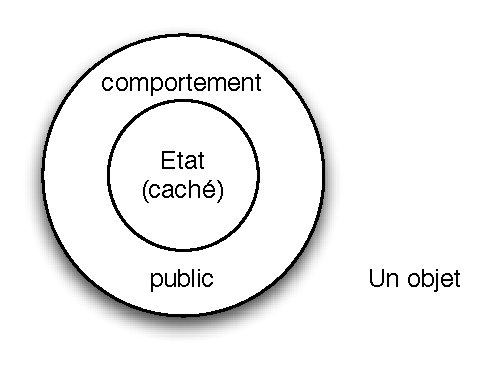
\includegraphics[scale=.5]{fig/encapsulation.pdf}
    \end{center}
  \end{figure}
\end{frame}

\subsubsection*{Encapsulation}

%%%%%%%%%%%%%%%%%%%%%%%%%%%%%%%%%%%%%%%%%%%%%
\begin{frame}{Principe d'encapsulation}
\begin{itemize}
	\item L'accès aux données (état) de l'objet ne peut être fait qu'au travers des méthodes
	\begin{itemize}
		\item les données sont \textbf{privées} (cachées)
		\item les méthodes \textbf{publiques} définissent l'\textbf{interface} de l'objet
	\end{itemize}
	\item Intérêt : la modification des structures de données n'affecte pas les programmes qui utiliseront l'objet
	\begin{itemize}
		\item masquage de l'implémentation : robustesse du code
		\item facilité d'évolution du logiciel
		\item pas de modification de l'interface
	\end{itemize}
\end{itemize}
\end{frame}

\subsubsection{Exemple}

% pour mémoire, ils ont déjà vu les string

\begin{frame}[fragile]
\frametitle{Déja vus : les objets \texttt{string}}
\begin{itemize}
\item Pas de vrai type chaîne de caractère en C
\item ALGPR : Utilisation du type \texttt{string} de C++
\item En réalité le type \texttt{string} est beaucoup plus puissant que l'utilisation faite l'an dernier
\end{itemize}
\begin{exampleblock}{Utilisation}
\begin{lstlisting}
string maChaine("toto");

cout << maChaine << endl;

string maChaine2 = "titi";

cout << maChaine2 << endl;

string maChaine3 = maChaine+maChaine2;

cout << maChaine3 << endl;
\end{lstlisting}
\end{exampleblock}
\end{frame}
%%%%%%%%%%%%%%%%%%%%%%%%%%%%%%%%%%%%%%%%%%%%%
\begin{frame}{{\href{code/Pendule.cxx}{\scalebox{.25}{
\includegraphics{fig/codeicon}}}} Exemple : un objet pendule}
  \begin{figure}[htbp]
    \begin{center}
      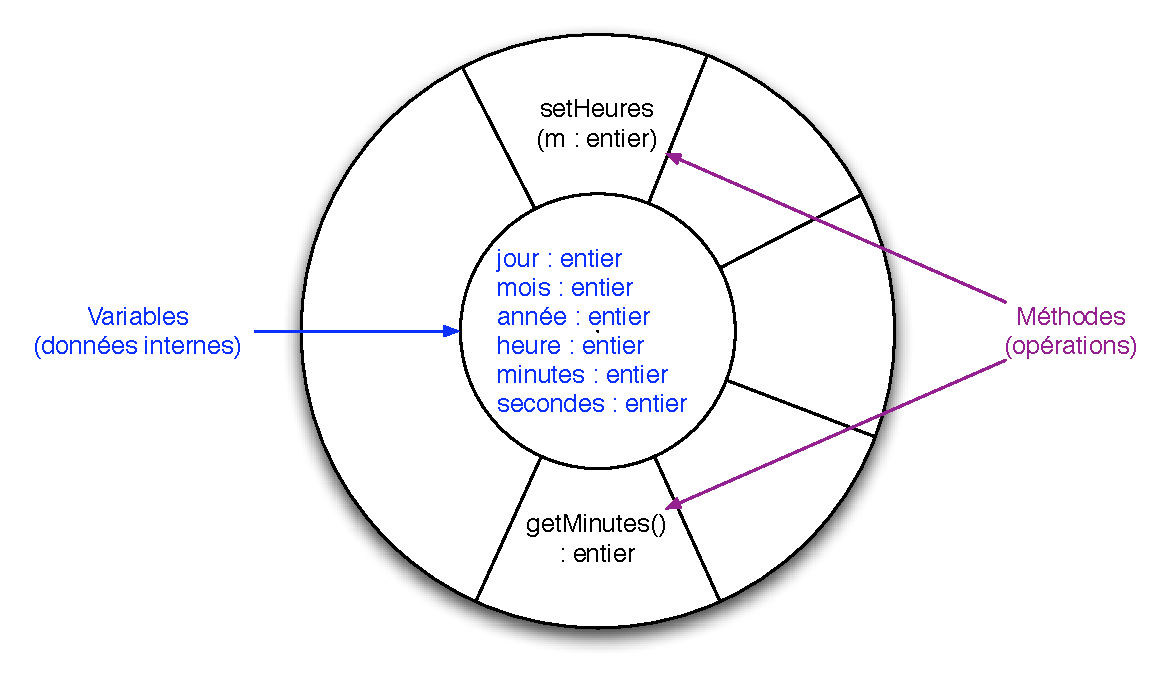
\includegraphics[scale=.45]{fig/encapsulation2.pdf}
    \end{center}
  \end{figure}
\end{frame}

\begin{frame}[fragile]
\frametitle{classe Pendule (1/2)}
\lstinputlisting[linerange=1-29]{code/pendule.cxx}
\end{frame}

\begin{frame}[fragile]
\frametitle{classe Pendule (2/2)}
\lstinputlisting[linerange=30-61]{code/pendule.cxx}
\end{frame}

\subsubsection*{Communication par messages}

%%%%%%%%%%%%%%%%%%%%%%%%%%%%%%%%%%%%%%%%%%%%%
\begin{frame}{Communication par messages}
\begin{block}{Communication}
Les objets \textbf{interagissent} et \textbf{communiquent} entre eux par l'envoi de \textbf{messages}
\end{block}
\begin{itemize}
\pause	\item Les méthodes publiques d'un objet correspondent aux messages que l'on peut lui envoyer
\pause	\item Les messages sont caractérisés par :
	\begin{itemize}
		\pause \item l'objet cible (récepteur) du message
		\pause \item le nom de la méthode à déclencher
		\pause \item les paramètres de cette méthode
	\end{itemize}
\end{itemize}
\end{frame}

%%%%%%%%%%%%%%%%%%%%%%%%%%%%%%%%%%%%%%%%%%%%%
\begin{frame}{\'Echange de messages}
\begin{center}
	Les objets s'envoient des messages entre eux
\end{center}
  \begin{figure}[htbp]
    \begin{center}
      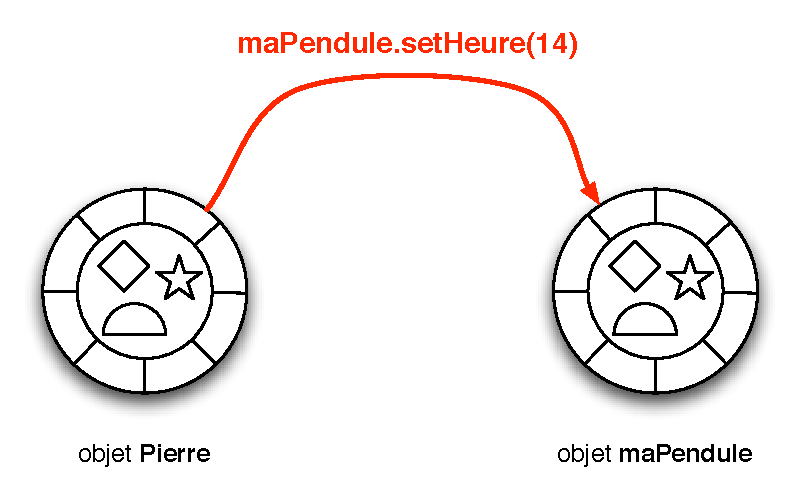
\includegraphics[scale=.55]{fig/messages.pdf}
    \end{center}
  \end{figure}
\end{frame}

\subsubsection*{Classes et instances}

%%%%%%%%%%%%%%%%%%%%%%%%%%%%%%%%%%%%%%%%%%%%%
\begin{frame}{Classes et instances}
\begin{itemize}
	\item Les objets (instances) sont créés (instanciés) à partir de <<moules>> qu'on appelle des \textbf{classes}
	\item classe = schéma, moule, modèle d'objets décrivant :
	\begin{itemize}
	\item partie privée : structure de données interne (attributs), corps des méthodes (algorithmes)
	\item partie publique (interface) : noms et paramètres des méthodes
	\end{itemize}
	\item la classe est un générateur d'objet : par \textbf{instanciation}, on peut fabriquer des objets (instances) respectant ce schéma/moule/modèle
\end{itemize}
\end{frame}

\begin{frame}{Vue duale}
\begin{itemize}
	\item Une \textbf{classe} est un \textbf{modèle} de définition pour des objets
	\begin{itemize}
		\item ayant même structure (même ensemble d'attributs)
		\item ayant même comportement (mêmes opérations, méthodes)
		\item ayant une sémantique commune
	\end{itemize}
	\item Les \textbf{objets} sont des représentations \textbf{dynamiques} (instanciation)
	<<vivantes>> du modèle défini pour eux au travers de la classe
	\begin{itemize}
		\item Une classe permet d'\textbf{instancier} (créer) plusieurs objets
		\item Chaque objet est \textbf{instance} d'une (seule) classe
	\end{itemize}
\end{itemize}
\end{frame}


%%%%%%%%%%%%%%%%%%%%%%%%%%%%%%%%%%%%%%%%%%%%%
\begin{frame}{Classes et instances}
\begin{center}
	La classe Pendule est le moule commun des deux objets
\end{center}
  \begin{figure}[htbp]
    \begin{center}
      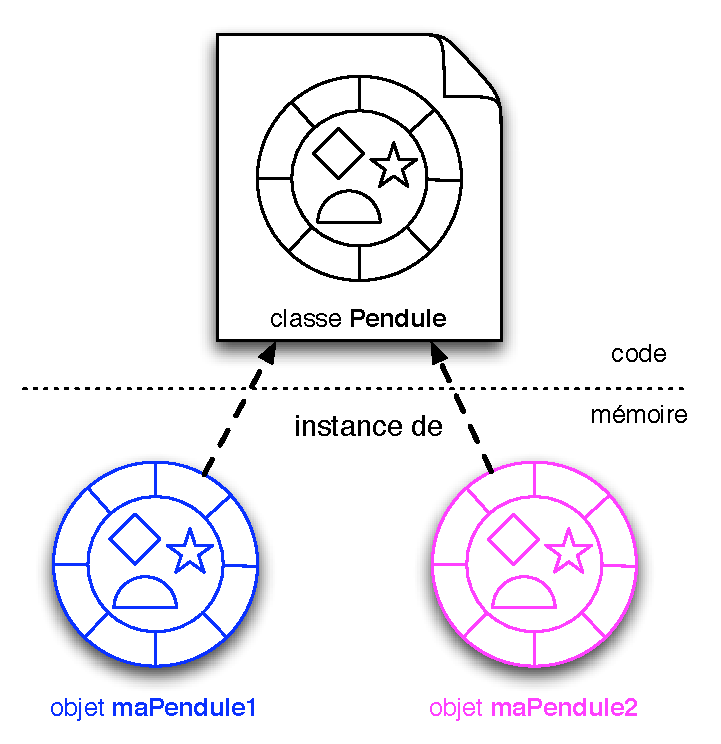
\includegraphics[scale=.37]{fig/instances.pdf}
    \end{center}
  \end{figure}
\end{frame}

\subsubsection*{Hiérarchie de classes}

%%%%%%%%%%%%%%%%%%%%%%%%%%%%%%%%%%%%%%%%%%%%%
\begin{frame}{Hiérarchie de classes}
\begin{itemize}
	\item les classes peuvent être des raffinements/spécialisations de classes existantes
	\item Elles forment alors une \textbf{hiérarchie de classes} où chaque classe :
	\begin{itemize}
		\item \textbf{hérite} des attributs et des méthodes de ses ancêtres (super-classe)
		\item ajoute de nouveaux attributs et/ou de nouvelles méthodes
		\item peut modifier ou redéfinir les méthodes héritées
	\end{itemize}
	\item Intérêt de l'héritage :
	\begin{itemize}
		\item réutilisation du code
		\item pas besoin de réinventer la roue à chaque fois
	\end{itemize}
\end{itemize}
\end{frame}

\begin{frame}{Hiérarchie de classes : exemple}
  \begin{figure}[htbp]
    \begin{center}
      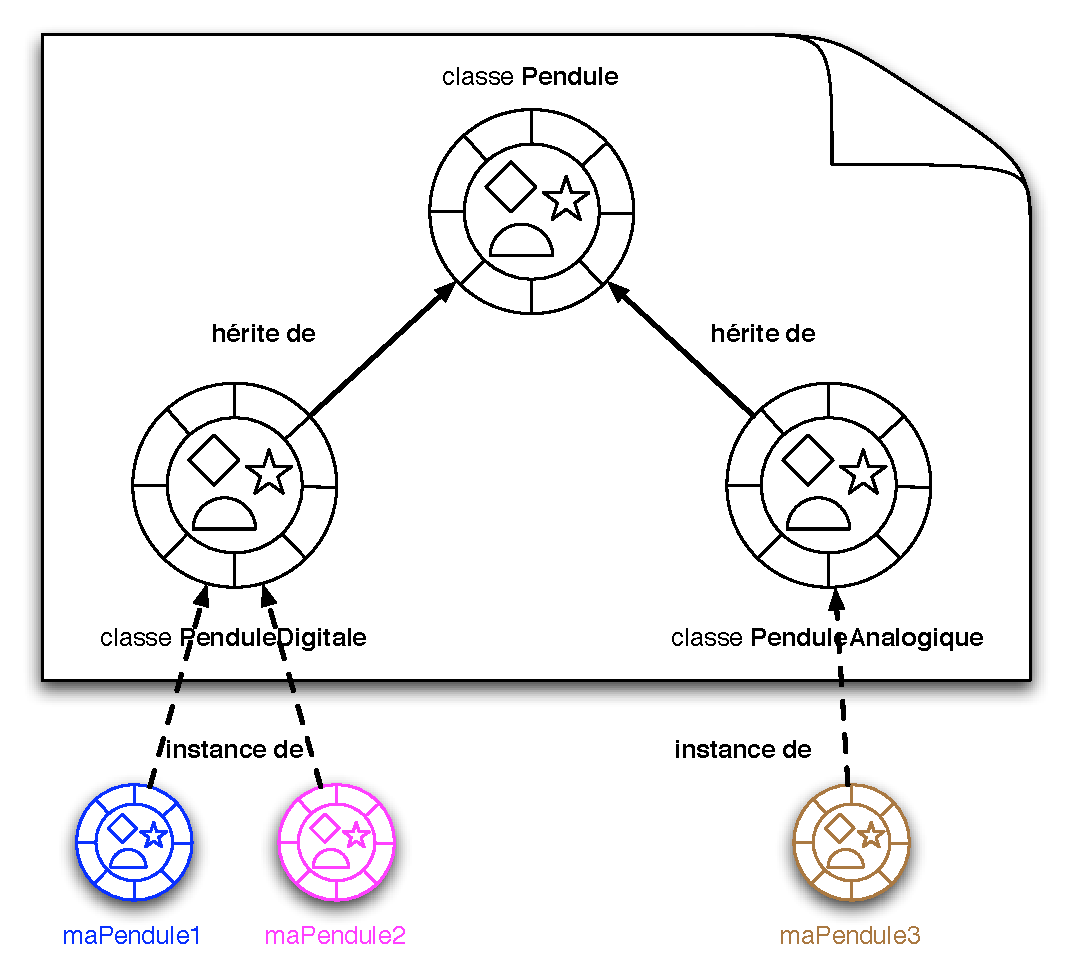
\includegraphics[scale=.32]{fig/heritage.pdf}
    \end{center}
  \end{figure}
\end{frame}

\subsection{Approche orientée-objet}

%%%%%%%%%%%%%%%%%%%%%%%%%%%%%%%%%%%%%%%%%%%%%
\begin{frame}{Approche orientée-objet}
\begin{itemize}
	\pause \item Rappel : approche procédurale
	\begin{itemize}
		\item Définir les structures de données
		\item Définir les traitements (analyse descendante)
		\item Le programme principal enchaîne les traitements
	\end{itemize}
	\pause \item Approche orientée-objet
	\begin{itemize}
		\item modéliser le monde de l'application avec des objets
	\end{itemize}
\end{itemize}
\end{frame}

\begin{frame}{Approche orientée-objet}
	\begin{itemize}
		\pause \item Identifier les classes
		\pause \item Pour chaque classe
		\begin{itemize}
			\item Définir son interface publique (quoi)
			\item Définir son implémentation (comment)
		\end{itemize}
		\pause \item Le programme principal
		\begin{itemize}
			\item création (instanciation) d'objets en mémoire
			\item lance l'exécution par envoi de messages aux objets créés
			\item ces messages peuvent provoquer d'autres envois de messages et/ou
			la création d'autres objets
		\end{itemize}
	\end{itemize}
\end{frame}

\subsection{Les classes en C++}

\begin{frame}{Déclaration de classe en C++}
\begin{definition}
\texttt{class} \textit{nom} \{ \\
...
\} ;
\end{definition}

\begin{itemize}
\item Attention : le point-virgule à la fin est obligatoire !
\item A l'intérieur de la classe :
\begin{itemize}
\item Attributs
\item Méthodes (ou déclaration de méthodes)
\item Indicateurs de protection
\end{itemize}
\end{itemize}
\end{frame}

\begin{frame}[fragile]
\frametitle{Déclaration des attributs}
\begin{definition}
\textit{type} \textit{nom}  ;
\end{definition}
\begin{itemize}
\item Le \textit{type} peut être un type de base ou un type objet
\item Si c'est un type objet, création d'une nouvelle instance
\end{itemize}
\begin{exampleblock}{Exemple}
\begin{lstlisting}
int jour;
Pendule maPendule;
string maChaine;
int *pJour;
\end{lstlisting}
\end{exampleblock}
\end{frame}

\begin{frame}[fragile]
\frametitle{Déclaration des méthodes}
\begin{itemize}
\item Déclaration et définition simultanées
\begin{definition}
\textit{typederetour} \textit{nom} ( \textit{listedeparamètrestypés} ) \{ \\
\texttt{// corps de la méthode} \\
\}
\end{definition}
\item Déclaration seule (classe dans un fichier .h)
\begin{definition}
\textit{typederetour} \textit{nom} ( \textit{listedeparamètrestypés} ) ;
\end{definition}
\item Définition (dans le fichier .cxx)
\begin{definition}
\textit{typederetour} \texttt{\textit{nomdeclasse}::\textit{nom}} ( \textit{listedeparamètrestypés} ) \{ \\
\texttt{// corps de la méthode} \\
\}
\end{definition}
\end{itemize}
\end{frame}

\begin{frame}[fragile]
\frametitle{classe exemplemeth1 : un seul fichier}
\lstinputlisting{code/exemplemeth1.cxx}
\end{frame}

\begin{frame}[fragile]
\frametitle{classe exemplemeth2 : deux fichiers}
\lstinputlisting{code/exemplemeth2.h}
\end{frame}

\begin{frame}[fragile]
\frametitle{classe exemplemeth2 : deux fichiers}
\lstinputlisting{code/exemplemeth2.cxx}
\end{frame}

\begin{frame}[fragile]
\frametitle{Exécution}
\begin{block}{Résultat d'exécution}
{\tiny \begin{verbatim}
[MacBook-Pro-de-Guillaume-2:optionRV/CPLUS/code] moreau% Debug/exemplemeth1
2
3
a = 2
b = 3
5
[MacBook-Pro-de-Guillaume-2:optionRV/CPLUS/code] moreau% Debug/exemplemeth2
2
3
a = 2
b = 3
5
\end{verbatim}}
\end{block}
\end{frame}

\begin{frame}{1 ou 2 fichiers ?}
\begin{itemize}
\item En réalité, la question est : déclaration seule ou déclaration+définition ?
\item Réponse technique : on peut mixer les deux
\item Réponse \textit{bonnes pratiques}
\begin{itemize}
\item Privilégier le découpage en plusieurs fichiers pour permettre le travail à plusieurs
\item Exception possible : les méthodes très très courtes et peu susceptibles d'être modifiées
\item Rappel : modifier un \texttt{.h} implique de recompiler tous les fichiers qui l'incluent (pas que directement)
\end{itemize}
\end{itemize}
\end{frame}

\begin{frame}[fragile]
\frametitle{Classe en deux parties : comment (bien) procéder ?}
\begin{enumerate}
\item Construire le \texttt{.h}, le fichier d'entête avec attributs et déclarations de méthodes
\item Encadrer le code par des macros
\begin{itemize}
\item S'assurer que le code ne sera inclus qu'une fois !
\end{itemize}
\begin{lstlisting}
#ifndef rvcpp_exemplemeth2_h
#define rvcpp_exemplemeth2_h
...
#endif
\end{lstlisting}
\item ou \texttt{\#pragma once} en début de chaque fichier .h
\item Inclure le \texttt{.h} dans le \texttt{.cxx}
\begin{lstlisting}
#include "exemplemeth2.h"
\end{lstlisting}
\item Ecrire les méthodes
\begin{itemize}
\item Attention au nom d'une méthode à l'extérieur de la classe !
\end{itemize}
\begin{lstlisting}
void exemplemeth2::methode1(int a, int b)
\end{lstlisting}
\end{enumerate}
\end{frame}

\begin{frame}{Classes en deux parties : problème classique}
\begin{itemize}
\item Cas simple : une classe a besoin d'une autre
\begin{enumerate}
\item Faire attention à l'ordre des include
\item utiliser la \textit{pré-déclaration} (forward declaration)
\end{enumerate}
\item Cas plus complexe
\begin{itemize}
\item Deux classes \textit{A} et \textit{B}, \textit{A} contenant un pointeur vers \textit{B} et \textit{B} un pointeur vers \textit{A}
\item La méthode précédente ne fonctionne plus
\item Seule la pré-déclaration peut fournir une solution
\end{itemize}
\end{itemize}
\end{frame}

\begin{frame}[fragile]
\frametitle{Cas problématique}
\begin{exampleblock}{Première classe}
\begin{lstlisting}
#ifndef rvcpp__classA_h
#define rvcpp__classA_h

class TwoClassA {
private:
    TwoClassB * ptrB;
public:
    void doSomething();
};

#endif
\end{lstlisting}
\end{exampleblock}
\begin{block}{Seconde classe}
\begin{lstlisting}
#ifndef rvcpp__classB_h
#define rvcpp__classB_h

class TwoclassB {
private:
    TwoclassA *ptrA;
};

#endif
\end{lstlisting}
\end{block}
\end{frame}

\begin{frame}[fragile]
\frametitle{Comment inclure ces classes ?}
\begin{itemize}
\item Si on inclut \textit{A} avant \textit{B}, erreur de compilation (et vice-versa)
\item Une solution
\begin{itemize}
\item Utiliser la pré-déclaration de \textit{B} juste avant celle de \textit{A}
\begin{lstlisting}
class TwoClassB;
\end{lstlisting}
\end{itemize}
\end{itemize}
\begin{exampleblock}{Déclaration de \textit{A}}
\begin{lstlisting}
#ifndef rvcpp__classA_h
#define rvcpp__classA_h

// forward declaration: can use TwoClassA pointers and references only
class TwoClassB;

class TwoClassA {
private:
    TwoClassB * ptrB;
public:
    void doSomething();
};

#endif
\end{lstlisting}
\end{exampleblock}
\end{frame}

\begin{frame}[fragile]
\frametitle{Utilisation de la classe A}
\begin{exampleblock}{TwoClassA.cxx}
\begin{lstlisting}
#include "2classA.h"
// with only A declared, it is not possible to use B in a complete way

void TwoClassA::doSomething() {
    // do something
}

int main() {
    // do nothing
}
\end{lstlisting}
\end{exampleblock}
\end{frame}

\begin{frame}{L'ordre des inclusions}
\begin{itemize}
\item Quelques bons principes
\begin{itemize}
\item Ne \textbf{jamais} inclure des .cxx
\item Ne pas renoncer à la modularité
\item N'inclure que ce qui est nécessaire (temps de compilation)
\end{itemize}
\item Quelques questions à se poser
\begin{itemize}
\item Inclure du plus général (libs standards) au plus particulier (ses propres fichiers) ? ou l'inverse ?
\begin{itemize}
\item première approche : Large-Scale C++ Software Design, J. Lakos. Addison-Wesley
\item seconde approche : Google C++ Style Guide : \url{http://google-styleguide.googlecode.com/svn/trunk/cppguide.xml}

\end{itemize}
\item Construire un fichier \texttt{includethemall.h} qui fait toutes les bonnes inclusions dans le bon ordre une fois pour toutes ?
\begin{itemize}
	\item C'est la méthode Visual Studio (stdafx.h et entêtes pré-compilées)
\end{itemize}
\end{itemize}
\end{itemize}
\end{frame}

% protection et exemple
\begin{frame}{Parties publiques et privées d'une classe : vue depuis C++}
\begin{itemize}
\item On a vu que les attributs d'un objet avaient vocation à être privés, tandis que certaines méthodes ont vocation à être publiques (l'interface de l'objet ou la liste des messages qu'il peut recevoir)
\item Définition des droits d'accès dans une classe
\begin{itemize}
\item \texttt{public:} ce qui est déclaré après cette ligne est accessible depuis partout
\item \texttt{private:} ce qui est déclaré après cette ligne n'est accessible que depuis l'intérieur de l'objet
\end{itemize}
\end{itemize}
\end{frame}
\begin{frame}{Exemple en Gestion bancaire : le compte client}
\begin{itemize}
	\item Que contient un compte (version simplifiée) ?

\begin{itemize}
	\item un numéro (c'est un entier)
	\item un solde (c'est un réel)
	\item une éventuelle interdiction bancaire (booléen)
\end{itemize}

\item Que peut-on faire avec un compte bancaire ?
\begin{itemize}
	\item Connaître son solde
	\item Déposer et retirer de l'argent
	\item Savoir si un compte est interdit bancaire
\end{itemize}

\end{itemize}
\end{frame}

\begin{frame}{Exemple en Gestion bancaire: le compte client}
\begin{itemize}
	\item Un enregistrement (\texttt{struct} en C) et des fonctions répondent-ils aux questions posées ?
	\item Pas complètement car:

\begin{itemize}
	\item il est interdit de modifier directement le solde
	\item on ne doit pas modifier le numéro d'un compte client
	\item seules certaines personnes sont habilitées à faire des opérations sur un compte
\end{itemize}

\item d'où la protection des données proposées par les mécanismes objets
\end{itemize}
\end{frame}

\begin{frame}{Exemple: La classe {\tt CompteClient} dans une banque (1/2)}
\vspace*{-4mm}
  \begin{figure}[htbp]
    \begin{center}
      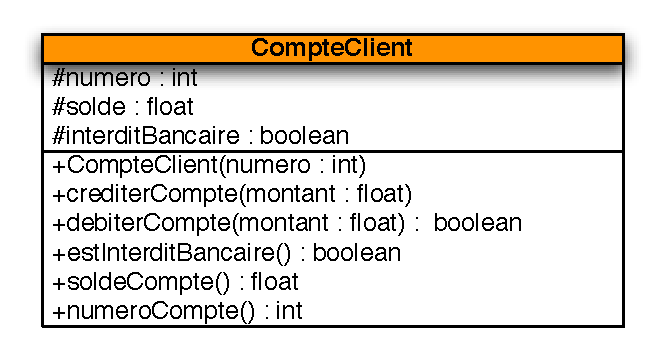
\includegraphics[scale=0.5]{fig/CompteClient.pdf}
    \end{center}
  \end{figure}
\vspace*{-6mm}
\begin{itemize}
	\item \emph{Encapsulation}: on a séparé les données des fonctions qui les manipulent, tout en conservant une seule entité, l'objet
	\item \emph{Protection}: on a protégé le {\tt solde}, dont la valeur ne peut être lue que par la méthode {\tt soldeCompte()}, et non modifiée\\ {\small sauf en ajoutant une méthode \textit{affecterCompte(x:float):void}.
}
\end{itemize}
\vspace*{-4mm}
\end{frame}

\begin{frame}{Exemple: La classe {\tt CompteClient} dans une banque (2/2)}
  \begin{figure}[htbp]
    \begin{center}
      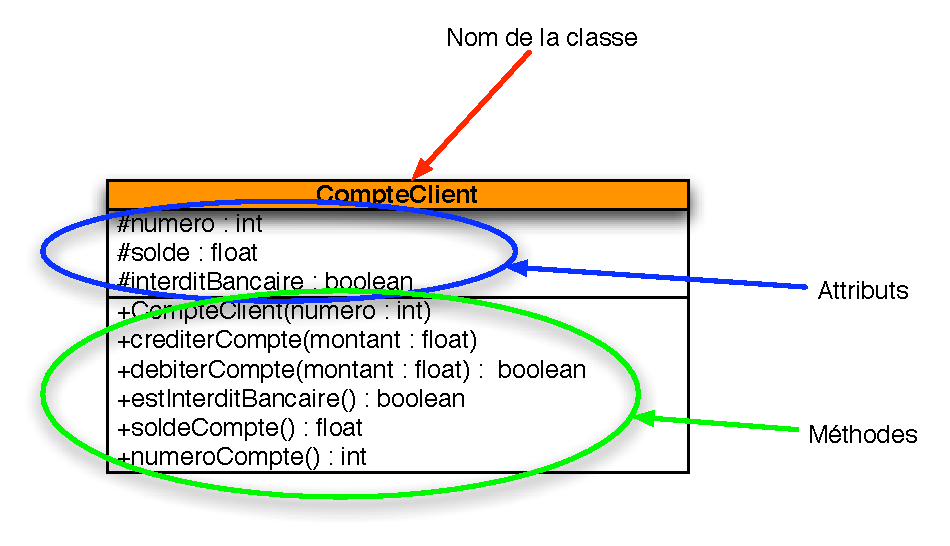
\includegraphics[scale=.4]{fig/CompteClientExplique.pdf}
    \end{center}
  \end{figure}

\end{frame}

% SSSSSSSSSSSSSSSSSSSSSSSSSSSSSSSSSSSSSSSSSSSSSS
\begin{frame}{Classes, instances...}
  \begin{figure}[htbp]
    \begin{center}
      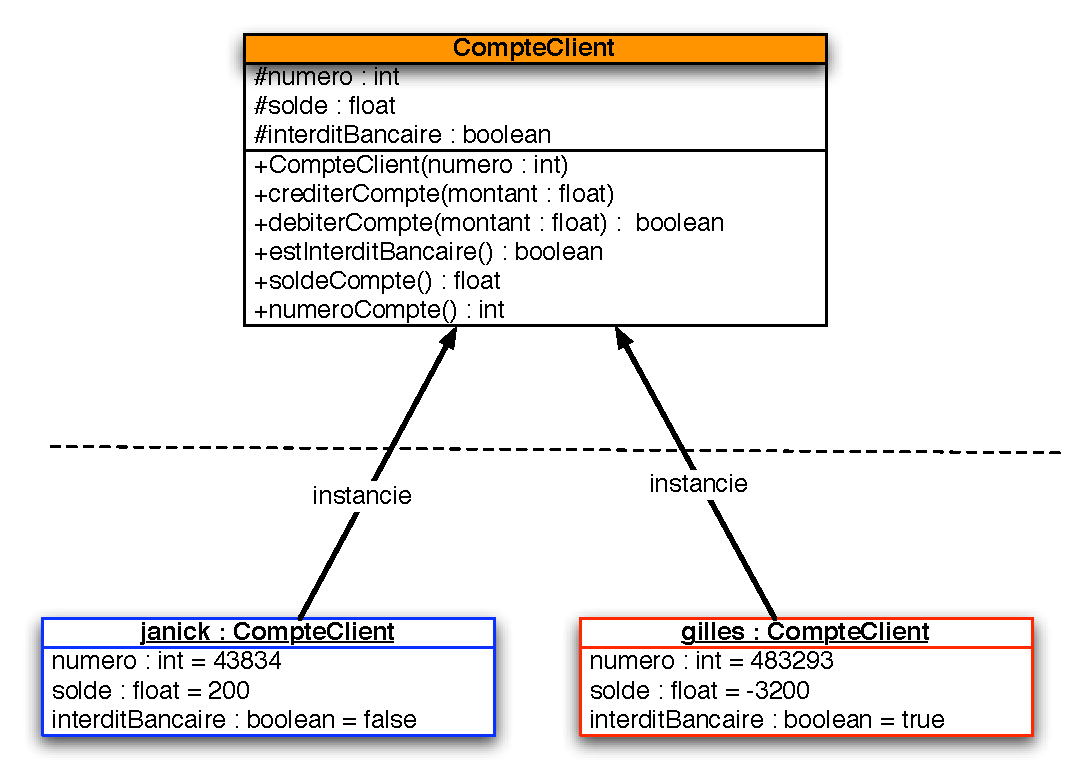
\includegraphics[scale=0.4]{fig/CompteClientInstance.pdf}
    \end{center}
  \end{figure}
\end{frame}

% constructeur & destructeur
%% cela pose d'autres questions : création et destruction d'un compte
\begin{frame}{Création d'un compte client}
\begin{itemize}
	\item Constat : on ne peut pas modifier le numéro d'un compte !
	\item la création d'un compte est une opération particulière qui doit :

\begin{itemize}
	\item définir de façon définitive le numéro du compte
	\item initialiser le solde du compte (à 0 généralement)
	\item mettre la variable \emph{interditBancaire} à faux
\end{itemize}
\item Les langages objet fournissent une méthode particulière : le \emph{constructeur}
\item Certains (dont C++) fournissent aussi un \emph{destructeur}
\end{itemize}
\end{frame}

\begin{frame}{Constructeurs et desctructeurs}
\begin{itemize}
\item Constructeur
\begin{itemize}
	\item Un constructeur est une fonction membre spéciale dont le nom est forcément celui de la classe
	\item Un constructeur n'a pas de type
	\item Une classe comporte généralement plusieurs constructeurs (en utilisant la surcharge, cf.  p.\ref{sec:surcharge})
	\item En fonction du nombre et du type des arguments passés, le constructeur approprié sera choisi
\end{itemize}
\item Destructeur
\begin{itemize}
\item Un destructeur est une fonction membre spéciale dont le nom est forcément un tilde ($\textasciitilde$) suivi du nom de la classe
\item Un destructeur n'a pas de type de retour ni d'argument
\end{itemize}
\end{itemize}
\end{frame}

\begin{frame}[fragile]
\frametitle{compte.h}
\begin{lstlisting}
#ifndef rvcpp_compte_h
#define rvcpp_compte_h

class compte {
private:
    float solde;
    bool ib;
    int numero;

public:
    float getSolde();
    int getNumero();

    void crediter(float montant);
    bool debiter(float montant);

    // constructeurs
    compte(int numero);

    // destructeur
    ~compte();
};

#endif
\end{lstlisting}
\end{frame}

\begin{frame}[fragile]
\frametitle{compte.cxx}
\begin{lstlisting}
#include "compte.h"

int compte::getNumero() {
    return numero;
}

float compte::getSolde() {
    return solde;
}

void compte::crediter(float montant) {
    solde += montant;
}

bool compte::debiter(float montant) {
    if (!ib && solde>=montant) {
        solde -= montant;
        return true;
    }
    return false;
}

compte::compte(int _numero) {
    numero = _numero;
    solde = 0.0;
    ib = false;
}

compte::~compte() {
    //nothing to do
}
\end{lstlisting}
\end{frame}

\begin{frame}[fragile]
\frametitle{Utilisation}
\begin{lstlisting}
#include <iostream>
using namespace std;

#include "compte.h"

int main() {
    compte janick(65136);
    janick.crediter(2000.0);
    cout << "solde du compte janick : " << janick.getSolde() << endl;
    if (janick.debiter(1000.0)) {
        cout << "debit autorise" << endl;
    }
    else {
        cout << "operation interdite" << endl;
    }
    cout << "solde du compte janick : " << janick.getSolde() << endl;
    compte *thomas = new compte(45558);
    thomas->crediter(500);
    cout << "solde du compte thomas : " << thomas->getSolde() << endl;
    delete thomas;
}
\end{lstlisting}
\pause\begin{block}{Résultat}
\tiny\begin{verbatim}
solde du compte janick : 2000
debit autorise
solde du compte janick : 1000
solde du compte thomas : 500
\end{verbatim}
\end{block}
\end{frame}

\begin{frame}{Rappels : encapsulation}
\begin{itemize}
\item Principe d'\textit{encapsulation} : tous les attributs d'une classe
doivent toujours être privés
\item Cela signifie que que seules les méthodes internes y ont accès (et donc qu'elles font les modifications comme il faut)
\item En clair : on a accès aux commandes de la voiture, pas directement à ce qu'il y a sous le capot
\item Ce n'est pas qu'un concept, c'est mis en \oe uvre et forcé par le language
\begin{center}
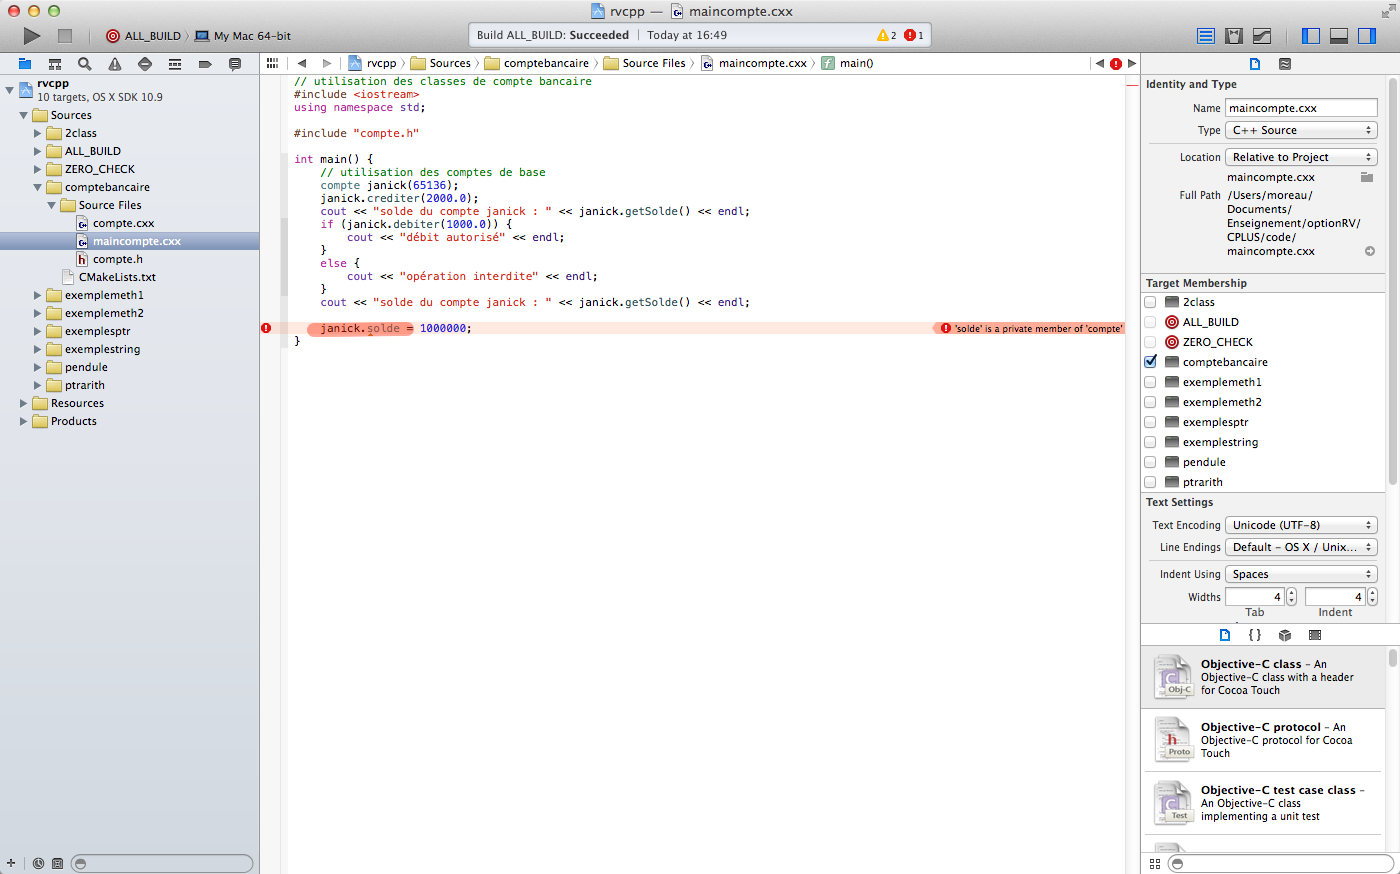
\includegraphics[width=\textwidth]{fig/encapsulation.png}
\end{center}
\end{itemize}
\end{frame}

\begin{frame}{Remarques}
\begin{itemize}
\item Nous reviendrons plus tard sur :
\begin{itemize}
\item Les protections
\item Les constructeurs et les destructeurs
\item La surcharge
\end{itemize}
\end{itemize}
\end{frame}

\begin{frame}[fragile]\frametitle{Interlude technique : les méthodes constantes}
\begin{itemize}
\item Une méthode constante est une méthode qui garantit ne pas altérer l'état d'un objet
\item On parle également de méthode en lecture seule
\item Déclaration :
\begin{itemize}
\item Le prototype de la méthode est suivi du mot-clé \texttt{const}
\item La déclaration de la méthode (dans le .cxx) est suivi de \texttt{const}, juste avant l'accolade de début
\end{itemize}
\item Utilité :
\begin{itemize}
\item Savoir ce que fait réellement une méthode (utilisation sans risque)
\item Optimisations du compilateur
\end{itemize}
\item Exemple : méthode \texttt{getSolde()} d'un compte bancaire
\begin{lstlisting}
float getSolde() const;

float compte::getSolde() const {
    return solde;
}
\end{lstlisting}
\end{itemize}
\end{frame}


% % Classes, mémoire et pointeurs

\begin{frame}[fragile]\frametitle{Gestion de la mémoire en C++ - les classes}

\begin{itemize}
\itemsep1pt\parskip0pt\parsep0pt
\item
  Que se passe-t-il lorsqu'une classe contient un élément d'un autre
  classe ?
\begin{lstlisting}
 class A {
 	B instB;
 };
\end{lstlisting}
\item
  En pratique l'instanciation de A créée automatiquement une instance de
  B dans la zone mémoire réservée pour l'instance de A.
\end{itemize}
\begin{columns}
\begin{column}{.6\textwidth}
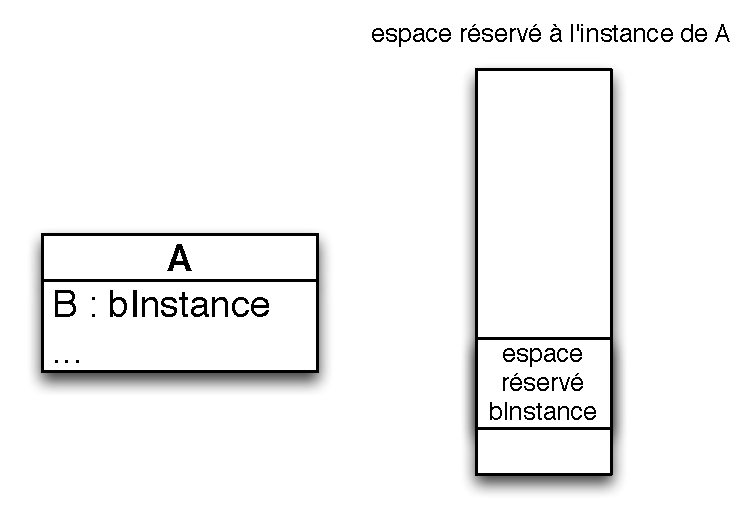
\includegraphics[width=6cm]{fig/inclusion-classe.pdf}
\end{column}
\begin{column}{.39\textwidth}
\begin{itemize}
\itemsep1pt\parskip0pt\parsep0pt
\item
  la destruction de A entraine la destruction de B
\end{itemize}
\end{column}
\end{columns}
\end{frame}


\begin{frame}[fragile]\frametitle{Gestion de la mémoire en C++ - les classes}

\begin{itemize}
\itemsep1pt\parskip0pt\parsep0pt
\item Utilisation d'un pointeur
\begin{lstlisting}
 class A {
 	B* instB;
 };
\end{lstlisting}
\item
  Les deux instances sont liées mais leur durée de vie est indépendante
\end{itemize}
\begin{columns}
\begin{column}{.6\textwidth}
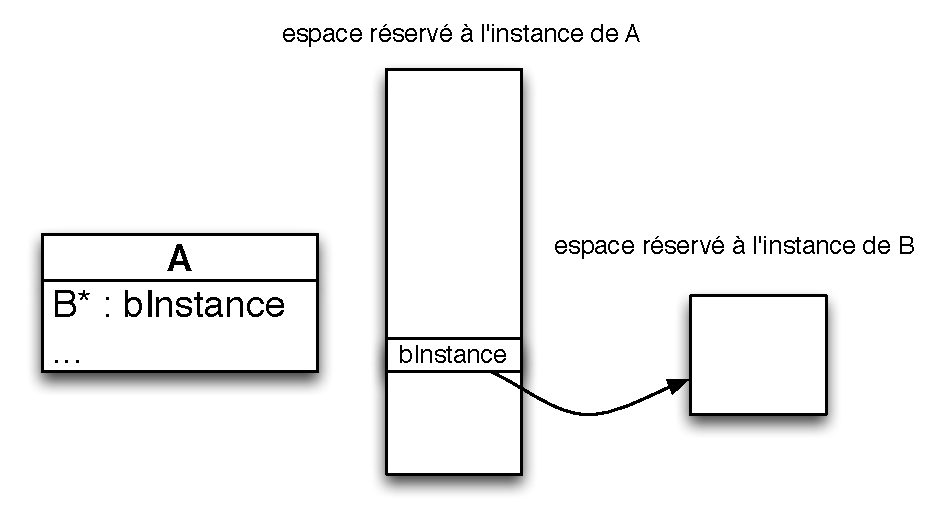
\includegraphics[width=6cm]{fig/inclusion-classeB.pdf}
\end{column}
\begin{column}{.39\textwidth}
\textbf{Exemple} de création/destruction de \textit{instB}

\begin{lstlisting}
A::A() {
	instB = new B();
}

A::~A() {
	delete instB;
}
\end{lstlisting}
\end{column}
\end{columns}
\end{frame}

\begin{frame}{Questions ?}

\begin{itemize}
\itemsep1pt\parskip0pt\parsep0pt
\item
  Pourquoi avoir écrit \textbf{exemple} au transparent précédent ?
\item
  Cycle de vie d'un objet vs un autre

  \begin{itemize}
  \itemsep1pt\parskip0pt\parsep0pt
  \item
    une question de génie de logiciel : B a-t-il une raison de survivre
    à A ?

    \begin{itemize}
    \itemsep1pt\parskip0pt\parsep0pt
    \item
      non : bouton appartenant à une fenêtre
    \item
      oui : un objet qui change de propriétaire (analogie jeu vidéo : un
      objet ramassé puis relâché)
    \end{itemize}
  \end{itemize}
\item
  Ok, mais C++ ne sait pas se débarrasser d'un objet tout seul

  \begin{itemize}
  \itemsep1pt\parskip0pt\parsep0pt
  \item
    Surtout si on utilise des pointeurs et des références
  \item
    On \textbf{doit} avoir une stratégie de gestion de la mémoire

    \begin{itemize}
    \itemsep1pt\parskip0pt\parsep0pt
    \item
      éviter l'utilisation de mémoire sans raison
    \item
      éviter d'utiliser un objet préalablement libéré
    \end{itemize}
  \item
    Cas typique : dans un contexte de gestion dynamique de la mémoire,
    on a une fonction qui retourne un objet

    \begin{itemize}
    \itemsep1pt\parskip0pt\parsep0pt
    \item
      qui se charge de l'allocation mémoire ? l'appelant, l'appelé ?
    \item
      qui est responsable de la libération de la mémoire ?
    \item
      attention aux créations d'objets temporaires
    \end{itemize}
  \end{itemize}
\end{itemize}

\end{frame}

\subsection{La surcharge}
\label{sec:surcharge}

\begin{frame}{Surcharge et redéfinition en C++}

\begin{itemize}
\itemsep1pt\parskip0pt\parsep0pt
\item
  principe : des fonctions qui portent le même nom
\item
  \textbf{surcharge} : plusieurs fonctions qui portent le même nom mais
  qui n'ont pas les mêmes paramètres (en nombre et/ou en type)

  \begin{itemize}
  \itemsep1pt\parskip0pt\parsep0pt
  \item
    le compilateur décide de la fonction à appeler en fonction du type
    des paramètres
  \item
    exemple : des fonctions \textit{max()} à respectivement 2, 3 ou 4 paramètres, des fonctions \textit{max()} s'appliquant à des types différents
  \item
    Cas particulier : surcharge des opérateurs
  \end{itemize}
\item
  \textbf{redéfinition} : plusieurs fonctions qui portent le nom et qui
  ont les mêmes paramètres

  \begin{itemize}
  \itemsep1pt\parskip0pt\parsep0pt
  \item
    utilisé plus tard pour l'héritage
  \end{itemize}
\end{itemize}

\end{frame}

\begin{frame}[fragile]\frametitle{Surcharge de fonctions}

\begin{itemize}
\itemsep1pt\parskip0pt\parsep0pt
\item
  Exemple : des fonctions qui calculent le maximum de plusieurs entiers
\item
  Ecriture ``C'' : une fonction \emph{max2(a,b)} , une fonction
  \emph{max3(a,b,c)}\ldots{}
\item
  Ecriture ``C++'' : toujours le même nombre de fonctions, mais elles
  portent toutes le même nom
\end{itemize}
\begin{lstlisting}
int max(int a,int b) {
    if (a>b) {
        return a;
    }
    else {
        return b;
    }
}

int max(int a,int b, int c) {
    return max(a,max(b,c));
}

int max(int a,int b, int c,int d) {
    return max(max(a,b),max(c,d));
}

int main() {
    cout << "max(2,4) = " << max(2,4) << endl;
    cout << "max(2,4,3) = " << max(2,4,3) << endl;
    cout << "max(6,4,5,7) = " << max(6,4,5,7) << endl;
}
\end{lstlisting}
\end{frame}

\begin{frame}{Cas particulier : surcharge des opérateurs}
\begin{itemize}
\item Les opérateurs sont des fonctions !
\begin{itemize}
\item Exemple : l'opérateur (binaire) d'addition est une fonction surchargée à deux paramètres de type \textit{t} et qui retourne un type \textit{t}
\item Elle pourrait s'écrire \texttt{int add(int a,int b)}
\item Inversement, une fonction de comparaison entre deux objets de type \textit{C} s'écrit \texttt{bool egalO(C const\& a, C const\&b)}
\item Autre possibilité, sous forme de méthode de la classe \textit{C} : \texttt{bool egal(const O\&a)}
\item On aimerait pouvoir l'écrire avec l'opérateur \texttt{==}
\end{itemize}
\end{itemize}
\end{frame}

\begin{frame}[fragile]\frametitle{Exemple : comparaison de deux nombres complexes}
\begin{itemize}
\item Déclaration des opérateurs (syntaxe forcée par la suite)
\begin{lstlisting}
class complexe1 {
private:
    double re;
    double im;

public:
...
    bool egal(complexe1 const& c1) const;
};

// operateurs externes
bool egal(complexe1 const&a,complexe1 const&b);
\end{lstlisting}
\item Définition
\begin{lstlisting}
bool complexe1::egal(complexe1 const& c1) const {
    if (re == c1.re && im == c1.im) {
        return true;
    }
    else {
        return false;
    }
}

bool egal(complexe1 const&a,complexe1 const&b) {
    return a.egal(b);
}
\end{lstlisting}
\end{itemize}
\end{frame}

\begin{frame}[fragile]\frametitle{Utilisation des fonctions}
\begin{itemize}
\item Code de test
\begin{lstlisting}
int main() {
    complexe1 c1,c2(2,3),c3(c2);
    cout << "c1 == c2 (interne) " << c1.egal(c2) << endl;
    cout << "c1 == c2 (externe) " << egal(c1,c2) << endl;
    cout << "c3 == c2 (interne) " << c3.egal(c2) << endl;
    cout << "c3 == c2 (externe) " << egal(c3,c2) << endl;

}
\end{lstlisting}
\begin{block}{Résultat}
{\tiny
\begin{verbatim}
c1 == c2 (interne) 0
c1 == c2 (externe) 0
c3 == c2 (interne) 1
c3 == c2 (externe) 1
\end{verbatim}
}
\end{block}
\item Comment écrire \texttt{c1 == c2} ?
\begin{itemize}
\item Utilisation d'un nouveau mot-clé : \texttt{operator}
\item La fonction associée à un opérateur \texttt{==} est \texttt{operator==()}
\end{itemize}
\end{itemize}
\end{frame}

\begin{frame}[fragile]\frametitle{Surcharge de l'opérateur \texttt{==}}
\begin{itemize}
\item Déclaration
\begin{lstlisting}
bool operator==(complexe1 const&a,complexe1 const&b);
\end{lstlisting}
\item Définition
\begin{lstlisting}
bool operator==(complexe1 const&a,complexe1 const&b) {
    return a.egal(b);
}
\end{lstlisting}
\item Utilisation
\begin{lstlisting}
    cout << "c1 == c2 (==) " << (c1 == c2) << endl;
    cout << "c3 == c2 (==) " << (c3 == c2) << endl;
\end{lstlisting}
\begin{block}{Résultat}
{\tiny
\begin{verbatim}
c1 == c2 (==) 0
c3 == c2 (==) 1
\end{verbatim}
}
\end{block}
\item A vous de faire de même avec l'opérateur \texttt{!=}
\end{itemize}
\end{frame}

\begin{frame}[fragile]\frametitle{Surcharge de l'opérateur \texttt{!=}}
\begin{itemize}
\item Déclaration
\begin{lstlisting}
bool operator!=(complexe1 const&a,complexe1 const&b);
\end{lstlisting}
\item Définition
\begin{lstlisting}
bool operator!=(complexe1 const&a,complexe1 const&b) {
    return !a.egal(b);
}
\end{lstlisting}
\item Utilisation
\begin{lstlisting}
    cout << "c1 != c2 " << (c1 != c2) << endl;
    cout << "c3 != c2 " << (c3 != c2) << endl;
\end{lstlisting}
\begin{block}{Résultat}
{\tiny
\begin{verbatim}
c1 != c2 1
c3 != c2 0
\end{verbatim}
}
\end{block}
\item Remarques
\begin{itemize}
\item Pourquoi avoir réutilisé le code existant ?
\item Fonction externe et encapsulation...
\end{itemize}
\end{itemize}
\end{frame}

\begin{frame}[fragile]\frametitle{Le cas de l'addition}
\begin{itemize}
\item Idée \textit{naturelle}
\begin{lstlisting}
complexe1 operator+(complexe1 const&c1,complexe1 const&c2);
\end{lstlisting}
\item Implémentation
\begin{itemize}
\item encapsulation = pas d'accès direct aux variables membres, lourdeur syntaxique
\item passer par une fonction \textit{amie} : rupture du principe d'encapsulation
\item passer par une méthode
\begin{itemize}
\item Soit par délégation
\item Soit par analogie avec l'opérateur unaire : \texttt{a += 5}
\item Une approche véritablement objet
\end{itemize}
\end{itemize}
\end{itemize}
\end{frame}

\begin{frame}[fragile]\frametitle{Surcharge de l'opérateur \texttt{+=}}
\begin{itemize}
\item Déclaration
\begin{lstlisting}
    void operator+=(complexe1 const&c1);
\end{lstlisting}
\item Définition
\begin{lstlisting}
void complexe1::operator+=(complexe1 const&c1) {
    re += c1.re;
    im += c1.im;
}
\end{lstlisting}
\item Utilisation
\begin{lstlisting}
    c2 += c3;
\end{lstlisting}
\begin{block}{Résultat}
{\tiny
\begin{verbatim}
2+3i + 2+3i = 4+6i
\end{verbatim}
}
\end{block}
\item Remarques
\begin{itemize}
\item Pour bien faire, l'opérateur devrait retourner un \texttt{complexe1\&}
\item Utilisation de \texttt{this}
\end{itemize}
\end{itemize}
\end{frame}

\begin{frame}[fragile]\frametitle{Surcharge de l'opérateur \texttt{+}}
\begin{itemize}
\item Déclaration
\begin{lstlisting}
complexe1 operator+(complexe1 const& c1,complexe1 const& c2);
\end{lstlisting}
\item Définition
\begin{lstlisting}
complexe1 operator+(complexe1 const& c1,complexe1 const &c2) {
    complexe1 c3(c1);
    c3 += c2;
    return c3;
}
\end{lstlisting}
\item Utilisation
\begin{lstlisting}
    c = a+b;
    t = t1+t2+t3;
\end{lstlisting}
\begin{block}{Résultat}
{\tiny
\begin{verbatim}
3+4i + 3+2i = 6+6i
23+3i + 3+5i + 2+1i = 28+9i
\end{verbatim}
}
\end{block}
\item A vous de jouer : ajout d'un complexe et d'un réel !
\end{itemize}
\end{frame}

\begin{frame}{Autres opérateurs surchargeables}

\begin{itemize}
\itemsep1pt\parskip0pt\parsep0pt
\item
  opérateurs mathématiques

  \begin{itemize}
  \itemsep1pt\parskip0pt\parsep0pt
  \item
    opérateurs binaires : +,-,*,/,\%
  \item
    opérateurs unaires : +=,-=,*=,/=,\%=
  \end{itemize}
\item
  opérateurs logiques

  \begin{itemize}
  \itemsep1pt\parskip0pt\parsep0pt
  \item
    bits à bits : \^{}, \textbar{}, \&, \textasciitilde{},
    \textless{}\textless{}, \textgreater{}\textgreater{} (et leur
    version unaire)
  \item
    relationnels : ==, !=, \textless{}, \textgreater{}, \textless{}=,
    \textgreater{}=
  \item
    logiques : !, \&\&, \textbar{}\textbar{}
  \end{itemize}
\item
  mais aussi

  \begin{itemize}
  \itemsep1pt\parskip0pt\parsep0pt
  \item
    opérateur d'affectation =
  \item
    opérateur d'accès tableau {[}{]}
  \item
    opérateur d'appel de fonction ()
  \item
    opérateur de gestion des adresses : \&, * et -\textgreater{}
  \end{itemize}
  \item Certains sont plus dangereux que d'autres...
\end{itemize}

\end{frame}

\begin{frame}{Autres opérateurs surchargeables (suite)}

\begin{itemize}
\itemsep1pt\parskip0pt\parsep0pt
\item
  Les opérateurs de gestion de mémoire (new, new{[}{]}, delete,
  delete{[}{]})
\item
  l'opérateur de séparation d'une liste , (utilité ??)
\item
  les opérateurs de conversion
\item
  Certains opérateurs ne \textbf{peuvent (quand même) pas} être
  surchargés

  \begin{itemize}
  \itemsep1pt\parskip0pt\parsep0pt
  \item
    l'opérateur ternaire ? :
  \item
    sélection d'un membre ., .*
  \item
    opérateur de résolution de portée ::
  \item
    \texttt{sizeof}
  \item
    \texttt{typeid}
  \end{itemize}
\item
  De façon générale, la surcharge des opérateurs est à utiliser

  \begin{itemize}
  \itemsep1pt\parskip0pt\parsep0pt
  \item
    avec parcimonie (on ne travaille pas tout seul)
  \item
    pour l'extension des opérations communes à de nouveaux types
  \item
    avec la même sémantique qu'avant la surcharge

    \begin{itemize}
    \itemsep1pt\parskip0pt\parsep0pt
    \item
      typiquement ne pas transformer un + en - !
    \end{itemize}
  \end{itemize}
\end{itemize}

\end{frame}

\begin{frame}[fragile]
\frametitle{Cas particulier intéressant : surcharge de l'opérateur
\texttt{\textless{}\textless{}}}

\begin{itemize}
\itemsep1pt\parskip0pt\parsep0pt
\item
  Pourquoi faire ?

  \begin{itemize}
  \itemsep1pt\parskip0pt\parsep0pt
  \item
    afficher des infos relatives à un objet qu'on a défini

    \begin{itemize}
    \itemsep1pt\parskip0pt\parsep0pt
    \item
      via un simple \texttt{cout} par exemple
    \end{itemize}
  \item
    sauver (et plus tard recharger) à partir d'un fichier
  \end{itemize}
\item
  Comment ?

  \begin{itemize}
  \itemsep1pt\parskip0pt\parsep0pt
  \item
    Plus tard : gestion des flux en C++
  \item
    Maintenant : surcharge simple et utilisation avec \texttt{cout}
  \item
    \texttt{\textless{}\textless{}} est bien un opérateur : ostream\&
    \texttt{operator\textless{}\textless{}(ostream\&,\emph{type} const\&)}
  \end{itemize}
\item
  Redéfinition pour le type complexe
\end{itemize}
\begin{lstlisting}
ostream& operator<<(ostream&s,complexe1 const&c) {
    s << c.getRe() << "+" << c.getIm() << "i";
    return s;
}
\end{lstlisting}
\end{frame}


\subsection{L'héritage en C++}


%%%%%%%%%%%%%%%%%%%%%%%%%%%%%%%%%%%%%%%%%%%%%%
\begin{frame}{Rappels : les classes}
\begin{itemize}
	\item Une classe représente une <<famille>> d'objets partageant les mêmes propriétés et méthodes
	\item Une classe sert à définir les propriétés des objets d'un type donné
	\begin{itemize}
		\item décrit l'ensemble des données et des opérations sur ces données
		\item elle sert de modèle pour la création d'objets (instances de la classe)
	\end{itemize}
\end{itemize}
\end{frame}

%%%%%%%%%%%%%%%%%%%%%%%%%%%%%%%%%%%%%%%%%%%%%%
\begin{frame}{Réutilisation : introduction}
\begin{itemize}
	\item Comment utiliser une classe comme une brique de base pour concevoir d'autres objets ?
	\item En conception objet, on définit des associations (relations) entre objets pour définir la réutilisation entre classes
	\item UML (Unified Modeling Language) définit toute une terminologie des associations possibles entre classes
	\begin{itemize}
		\item un des objectifs d'un cours de <<Génie Logiciel>> (option info par exemple)
		\item un objet fait appel à un autre $\longrightarrow$ délégation
		\item un objet peut être créé à partir d'un autre objet $\longrightarrow$ héritage
	\end{itemize}
\end{itemize}
\end{frame}

\subsection{Délégation}
\subsubsection*{Exemple}

%%%%%%%%%%%%%%%%%%%%%%%%%%%%%%%%%%%%%%%%%%%%%%
\begin{frame}[fragile]
\frametitle{Délégation}
\begin{itemize}
	\item Un objet \texttt{o1} membre de la classe \emph{C1} utilise les services d'un objet \texttt{o2} instance de la classe \emph{C2} (\texttt{o1} délègue une partie de son activité à \texttt{o2})
	\item La classe \emph{C1} utilise les services de la classe \emph{C2}
\begin{figure}[htbp]
    \begin{center}
      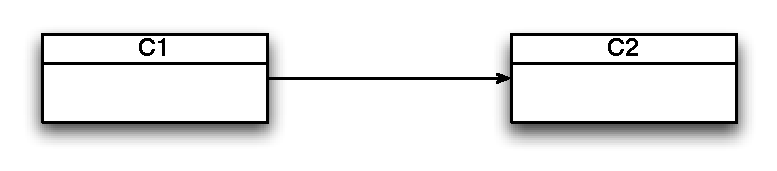
\includegraphics[scale=.5]{fig/delegation.pdf}
    \end{center}
  \end{figure}
  \item La classe cliente (\emph{C1}) utilise les services de la classe serveuse
\end{itemize}
\begin{block}{Schéma type}
\begin{lstlisting}[language=C++]
public class C1 {
private:
   C2 o2; // ou C2 *o2;
\end{lstlisting}
\end{block}
\end{frame}

%%%%%%%%%%%%%%%%%%%%%%%%%%%%%%%%%%%%%%%%%%%%%%
\begin{frame}[fragile]
\frametitle{Délégation : exemple}
\begin{itemize}
  \item Exemple de la classe \emph{Cercle}
  \begin{itemize}
  	\item rayon : un nombre réel
	\item centre : deux réels ou bien un \emph{Point}
  \end{itemize}
\end{itemize}
\begin{lstlisting}[language=C++]
public class Cercle {
private:
  Point centre; // ou Point *centre
  private double rayon;

public:
  Cercle(Point _centre, double _rayon) {
    centre = _centre;
    rayon = _rayon;
  }
};
\end{lstlisting}
\end{frame}

%%%%%%%%%%%%%%%%%%%%%%%%%%%%%%%%%%%%%%%%%%%%%%
\begin{frame}[fragile]
\frametitle{Délégation : exemple}
\begin{itemize}
	\item l'association entre les classes \emph{Cercle} et \emph{Point} exprime le fait qu'un cercle \textbf{possède} (a un) centre
	\item Le point représentant le centre a une existence autonome (cycle de vie indépendant
	\item Il peut être utilisé en dehors du cercle dont il est le centre !
	\begin{itemize}
		\item si on translate le cercle, on translate le point et tous les objets qui utilisent ce point
		\item Solution (en place) : effectuer une copie du point dans le constructeur
	\end{itemize}
\begin{lstlisting}[language=C++]
// cas Point centre
  centre = _centre; // dans les deux cas
// cas Point *centre
  centre = new Point(_centre);
\end{lstlisting}
%% note : les cycles de vie du cercle et du point sont maintenant liés : si le cercle est déplacé ou déruit
%% le point l'est aussi
\end{itemize}
\end{frame}

\subsubsection*{Agrégation / Composition}

%%%%%%%%%%%%%%%%%%%%%%%%%%%%%%%%%%%%%%%%%%%%%%
\begin{frame}{Agrégation / Composition}
\begin{itemize}
	\item L'exemple précédent traduit deux nuances (sémantiques) de l'association \textbf{a un} entre la classe \emph{Cercle} et la classe \emph{Point}
	\item UML distingue deux types de sémantique en définissant deux types de relations
\end{itemize}
\begin{figure}[htbp]
    \begin{center}
      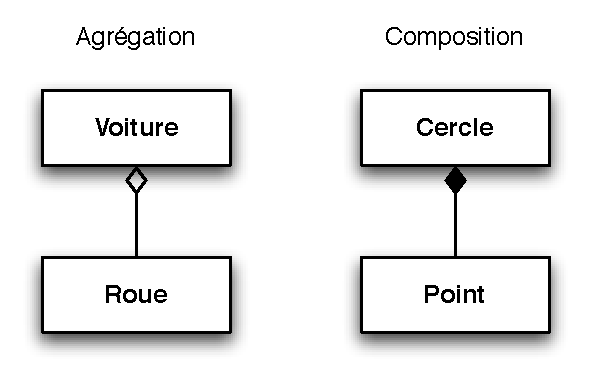
\includegraphics[scale=.45]{fig/agregcompo.pdf}
    \end{center}
  \end{figure}
\end{frame}

%%%%%%%%%%%%%%%%%%%%%%%%%%%%%%%%%%%%%%%%%%%%%%
\begin{frame}{Agrégation / Composition}
\begin{itemize}
	\item \textbf{Agrégation} : l'élément agrégé \emph{Roue} a un existence autonome en dehors de l'agrégat
	\item \textbf{Agrégation forte / composition} : à un même moment, une instance de composant \emph{Point} ne peut être liée qu'à un seul agrégat \emph{Cercle} et le composant a un cycle de vie dépendant de l'agrégat
	\begin{itemize}
	\item Pas vrai dans tous les cas, mais voulu et forcé ici !
	\end{itemize}
\end{itemize}
\end{frame}

\subsubsection*{Syntaxe}

%%%%%%%%%%%%%%%%%%%%%%%%%%%%%%%%%%%%%%%%%%%%%%
\begin{frame}{Héritage : exemple introductif}
\begin{itemize}
	\item Le problème :
	\begin{itemize}
		\item une application a besoin de services dont une partie seulement est proposée par une classe déjà définie
		\item ne pas réécrire le code
	\end{itemize}
\end{itemize}
\begin{figure}[htbp]
    \begin{center}
      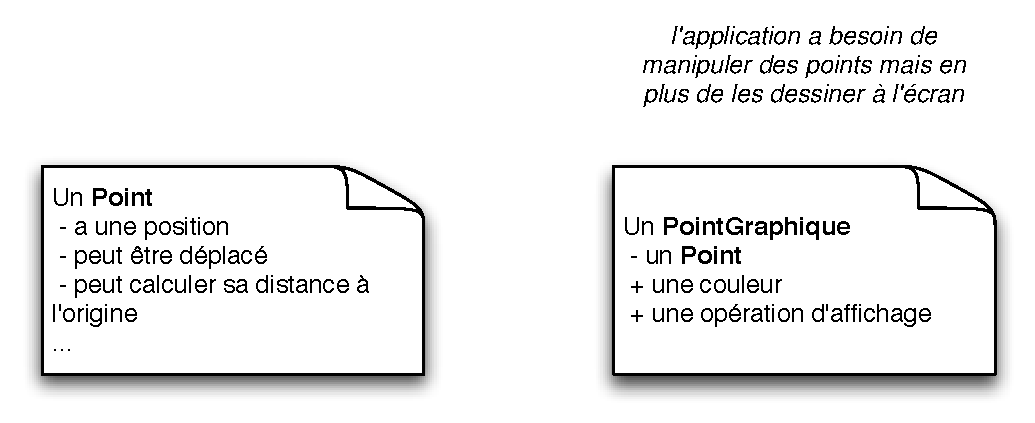
\includegraphics[scale=.42]{fig/pointgraphique.pdf}
    \end{center}
  \end{figure}
\end{frame}

%%%%%%%%%%%%%%%%%%%%%%%%%%%%%%%%%%%%%%%%%%%%%%
\begin{frame}{Pourquoi l'héritage plutôt que agrégation/composition ?}
\begin{itemize}
	\item par simplicité...
	\item ici, on réutilise les méthodes de {Point} dans {PointGraphique}
	\item éviter de rerouter tous les appels à \textit{deplacer()} de {PointGraphique} vers {Point}
	\item exemple opposé : création d'une pile à partir d'une liste
	\begin{itemize}
		\item on ne veut pas donner accès à toutes les méthodes de la liste
	\end{itemize}
\end{itemize}
\end{frame}

%%%%%%%%%%%%%%%%%%%%%%%%%%%%%%%%%%%%%%%%%%%%%%
\begin{frame}[fragile]
\frametitle{Héritage : syntaxe C++}
\begin{itemize}
	\item La classe \emph{PointGraphique} hérite de (elle étend) la classe \emph{Point}
	\begin{itemize}
		\item elle possède les variables et méthodes définies dans la classe \emph{Point} ($x$ et $y$)
		\item elle ajoute des attributs de couleur \texttt{r,g,b}
		\item elle définit une nouvelle méthode \texttt{dessine()}
	\end{itemize}
\end{itemize}
\begin{exampleblock}{Déclaration}
\begin{lstlisting}[language=C++]
class PointGraphique : public Point {
private:
    int r,g,b;

public:
    PointGraphique();
    PointGraphique(double _x,double _y,int _r,int _g, int _b);
    PointGraphique(double _x,double _y);

    void dessine();
};
\end{lstlisting}
\end{exampleblock}
\end{frame}

\begin{frame}[fragile]
\frametitle{Héritage : Ecriture des méthodes}
\begin{itemize}
	\item Seul le constructeur diffère !
	\item Il peut (doit) faire appel au constructeur de la classe \textit{Point}
	\item Syntaxe \texttt{\textit{Pointgraphique::PointGraphique( ) : Point( )}}
\end{itemize}
\begin{exampleblock}{Définition des méthodes}
\begin{lstlisting}[language=C++]
#include "point.h"
#include "pointgraphique.h"

PointGraphique::PointGraphique() : Point() {
    r = g = b = 255; // couleur par defaut = blanc
}

PointGraphique::PointGraphique(double _x,double _y,int _r,int _g, int _b)
 : Point(_x,_y), r(_r), g(_g), b(_b) {
    // plus rien a faire
}

PointGraphique::PointGraphique(double _x,double _y) : Point(_x,_y) {
    r = g = b = 255; // couleur par defaut = blanc
}
\end{lstlisting}
\end{exampleblock}
\end{frame}

%%%%%%%%%%%%%%%%%%%%%%%%%%%%%%%%%%%%%%%%%%%%%%%
\begin{frame}[fragile]
\frametitle{Utilisation des instances d'une classe héritée}
\begin{itemize}
	\item Un objet instance de \emph{PointGraphique} possède les attributs définis dans \emph{PointGraphique} ainsi que ceux définis dans \emph{Point}
	\item Un  objet instance de \emph{PointGraphique} répond aux messages définis par les méthodes décrites dans \emph{PointGraphique} et aussi à ceux définis dans les méthodes de \emph{Point}
\end{itemize}
\begin{exampleblock}{Utilisation}
\begin{lstlisting}[language=C++]
int main() {
    PointGraphique pg;

    pg.setX(5.5);
    pg.setY(2.3);
    pg.translater(2.0, 0.0);
    pg.setCouleur(128, 128, 0);

}
\end{lstlisting}
\end{exampleblock}
\end{frame}

%%%%%%%%%%%%%%%%%%%%%%%%%%%%%%%%%%%%%%%%%%%%%%%
\begin{frame}[fragile]
\frametitle{Résolution statique des messages}
\begin{figure}[htbp]
    \begin{center}
      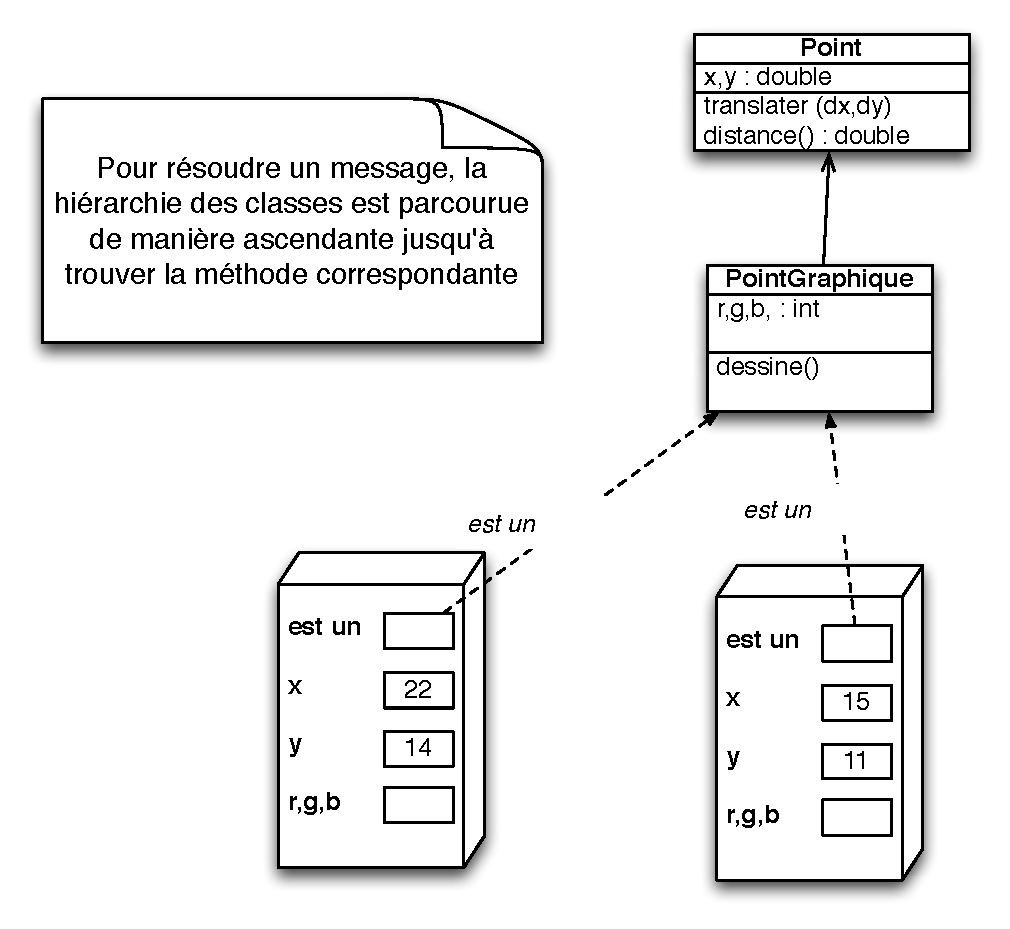
\includegraphics[scale=.42]{fig/resolution.pdf}
    \end{center}
  \end{figure}
\end{frame}

\subsubsection*{Terminologie}

%%%%%%%%%%%%%%%%%%%%%%%%%%%%%%%%%%%%%%%%%%%%%%
\begin{frame}{Terminologie de l'héritage}
\begin{itemize}
	\item L'\textbf{héritage} permet de reprendre les caractéristiques d'une classe $M$ existante pour les étendre et définir ainsi une nouvelle classe $F$ qui hérite de $M$
	\item les objets de $F$ possèdent toutes les caractéristiques de $M$ avec en plus celles définies dans $F$
	\begin{itemize}
		\item $M$ est la classe mère et $F$ la classe fille
		\item $F$ hérite de $M$
		\item $F$ est une sous-classe de $M$
		\item $M$ est la super-classe de $F$
	\end{itemize}
\end{itemize}
\end{frame}

%%%%%%%%%%%%%%%%%%%%%%%%%%%%%%%%%%%%%%%%%%%%%%
\begin{frame}{Généralisation / spécialisation}
\begin{figure}[htbp]
    \begin{center}
      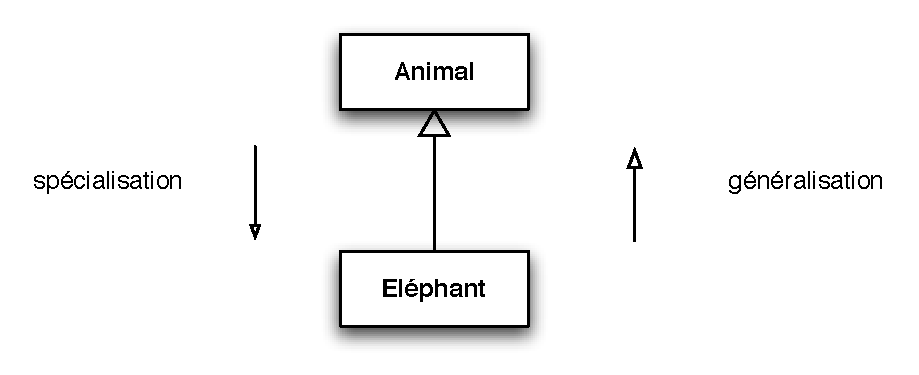
\includegraphics[scale=.45]{fig/genspe.pdf}
    \end{center}
  \end{figure}
\begin{itemize}
	\item la \textbf{généralisation} exprime la relation <<est-un>> entre une classe et sa super-classe
	\item la \textbf{spécialisation} exprime la relation de <<particularisation>> entre une classe et sa sous-classe
\end{itemize}
\end{frame}

%%%%%%%%%%%%%%%%%%%%%%%%%%%%%%%%%%%%%%%%%%%%%%%
\begin{frame}{Généralisation / spécialisation}
\begin{itemize}
	\item Utilisation de la spécialisation : \textbf{réutilisation} par modification incrémentielle des descriptions existantes
	\item Utilisation de la généralisation : \textbf{abstraction} par factorisation des propriétés communes aux sous-classes
	\item il n'y a pas de limitation dans le nombre de niveaux de la hiérarchie d'héritage
	\item les méthodes et les attributs sont automatiquement héritées au travers de tous les niveaux
\end{itemize}
\end{frame}

%\subsection{Redéfinition des méthodes}

%%%%%%%%%%%%%%%%%%%%%%%%%%%%%%%%%%%%%%%%%%%%%%
\begin{frame}{Redéfinition des méthodes}
\begin{itemize}
	\item une sous-classe peut \textbf{redéfinir} des méthodes dont elle hérite et fournir ainsi des implémentations spécialisées pour celles-ci
	\item lorsque la classe définit une méthode dont le nom, le type de retour et les arguments sont identiques à ceux d'une méthode dont on hérite
	\begin{itemize}
	\item On dit aussi qu'une méthode \textbf{masque} celle de la classe mère
	\end{itemize}
	\item Lorsqu'une méthode redéfinie par une classe est invoquée pour un objet de cette classe, c'est la nouvelle définition qui est invoquée
\end{itemize}
\end{frame}

%%%%%%%%%%%%%%%%%%%%%%%%%%%%%%%%%%%%%%%%%%%%%%%
\begin{frame}[fragile]
\frametitle{{\href{code/exheritageA.cxx}{\scalebox{.25}{
\includegraphics{fig/codeicon}}}} Redéfinition des méthodes : exemple (1/2)}
\begin{itemize}
\item Déclaration
\begin{lstlisting}[language=C++]
class exheritageA {
public:
    void hello();
    void affiche();

};

class exheritageB : public exheritageA {
public:
    void affiche();
};
\end{lstlisting}
\item Définition
\begin{lstlisting}
void exheritageA::hello() {
    cout << "hello" << endl;
}

void exheritageA::affiche() {
    cout << "je suis un objet de la classe exheritageA" << endl;
}

void exheritageB::affiche() {
    cout << "je suis un objet de la classe exheritageB" << endl;
}
\end{lstlisting}
\end{itemize}
\end{frame}
%
%%%%%%%%%%%%%%%%%%%%%%%%%%%%%%%%%%%%%%%%%%%%%%%
\begin{frame}[fragile,containsverbatim]
\frametitle{{\href{code/exheritageB.java}{\scalebox{.25}{
\includegraphics{fig/codeicon}}}}  Redéfinition des méthodes : exemple (2/2)}
\begin{lstlisting}[language=C++]
int main() {
    exheritageA a;
    exheritageB b;

    a.hello();
    b.hello();

    a.affiche();
    b.affiche();
}
\end{lstlisting}
\begin{itemize}
	\item produit l'affichage suivant
\end{itemize}
\pause \begin{block}{Résultat}
{\tiny \begin{verbatim}
hello
hello
je suis un objet de la classe exheritageA
je suis un objet de la classe exheritageB
\end{verbatim}}
\end{block}
\end{frame}
%
%
%%%%%%%%%%%%%%%%%%%%%%%%%%%%%%%%%%%%%%%%%%%%%%%
\begin{frame}{Redéfinition des méthodes}
\begin{itemize}
	\item Ne pas confondre redéfinition et surcharge !
\end{itemize}
\begin{figure}[htbp]
    \begin{center}
      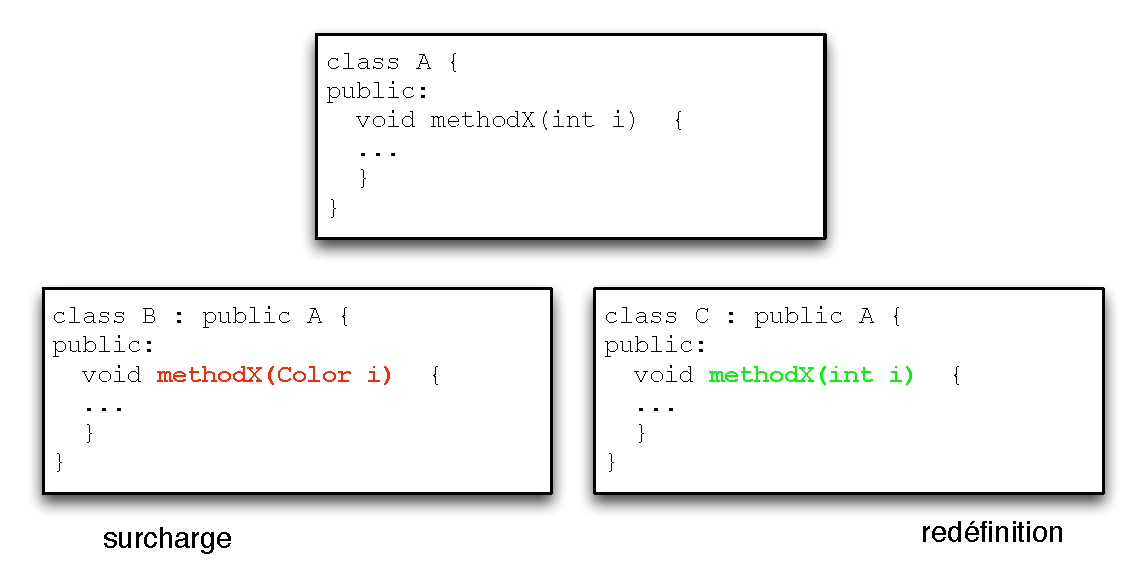
\includegraphics[scale=.45]{fig/rideload.pdf}
    \end{center}
  \end{figure}
\end{frame}
%
%%%%%%%%%%%%%%%%%%%%%%%%%%%%%%%%%%%%%%%%%%%%%%%
\begin{frame}[fragile]
\frametitle{{\href{code/heritageC.cxx}{\scalebox{.25}{
\includegraphics{fig/codeicon}}}}  Redéfinition avec réutilisation}
\begin{itemize}
	\item On peut réutiliser le code de la classe mère avec l'opérateur de résolution de portée \texttt{::}
	\item Exemple : Définition d'une classe \textit{exheritageC} similaire à \textit{exheritageB}
\end{itemize}
\begin{lstlisting}[language=C++]
void exheritageC::affiche() {
    exheritageA::affiche();
    cout << "je suis un objet de la classe exheritageC" << endl;
}

// extrait du main()
int main() {
...
    exheritageC c;
    c.affiche();
}
\end{lstlisting}
\pause \begin{block}{Résultat}
{\tiny \begin{verbatim}
je suis un objet de la classe exheritageA
je suis un objet de la classe exheritageC
\end{verbatim}}
\end{block}
\end{frame}

\subsubsection{Retour sur les protections}

\begin{frame}{Protection}

\begin{itemize}
\itemsep1pt\parskip0pt\parsep0pt
\item
  Situation actuelle

  \begin{itemize}
  \itemsep1pt\parskip0pt\parsep0pt
  \item
    \textbf{public} accessible depuis partout (sous réserve de disposer
    d'une instance de la classe)
  \item
    \textbf{private} accessible uniquement depuis l'intérieur (i.e.~les
    méthodes de la classe)
  \item
    problème : une classe dérivée ne peut accéder aux membres privés de
    sa classe mère
  \end{itemize}
\item
  Solution

  \begin{itemize}
  \itemsep1pt\parskip0pt\parsep0pt
  \item
    \textbf{protected} : accessible depuis l'intérieur de la classe et
    de toutes les classes dérivées
  \end{itemize}
\item
  Ce n'est pas tout

  \begin{itemize}
  \itemsep1pt\parskip0pt\parsep0pt
  \item
    notion de fonctions \textbf{friend}
  \item
    héritage via le mot-clé \textbf{public}\ldots{} il existe d'autres
    formes d'héritage
  \item
    classes internes
  \end{itemize}
\end{itemize}

\end{frame}

\subsubsection{Exemple}

\begin{frame}{Exemple : compte bancaire avec autorisation de découvert}
\begin{itemize}
\item Compte bancaire "standard" : notion forcément incomplète
\begin{itemize}
\item en pas uniquement en raison de nos simplifications
\end{itemize}
\item On peut avoir différents types de comptes bancaires
\item Exemple : certains comptes ont une autorisation de découvert, c'est-à-dire qu'on peut avoir un \textit{solde légèrement négatif}, dans une limite fixée par la banque
\item Nouvel attribut
\begin{itemize}
\item le montant du découvert autorisé
\end{itemize}
\item Méthodes
\begin{itemize}
\item modification de la méthode \textit{debiter()}
\item ajout d'un setter pour le montant du découvert autorisé
\item le reste est identique
\end{itemize}
\end{itemize}
\end{frame}

\begin{frame}[fragile]\frametitle{Exemple : le code (1/2)}
\begin{codeblock}{Déclaration de la classe}
\begin{lstlisting}
class comptead : public compte {
protected:
    float montant_ad;

public:
    bool debiter(float montant);
    void infos() const;
    void setMontantAD(float m);
    comptead(int numero);
};
\end{lstlisting}
\end{codeblock}
\end{frame}


\begin{frame}[fragile]\frametitle{Exemple : le code (2/2)}
\begin{codeblock}{Définition des méthodes}
\begin{lstlisting}
void comptead::setMontantAD(float m) {
    montant_ad = m;
}


bool comptead::debiter(float montant) {
    if (!ib && solde+montant_ad>=montant) {
        solde -= montant;
        return true;
    }
    return false;
}

comptead::comptead(int n) : compte(n) {
    montant_ad = 0.0;
}

void comptead::infos() const {
    compte::infos();
    cout << "montant de l'autorisation de decouvert : " << montant_ad << endl;
}
\end{lstlisting}
\end{codeblock}

\end{frame}
%\subsubsection{Héritage multiple}



\subsection{Le polymorphisme}

% % polymorphisme

\begin{frame}{Rappels : les classes}
\begin{itemize}
	\item La réutilisation est un aspect important de l'héritage, mais pas forcément le plus important !
	\item Le deuxième point fondamental est la relation qui lie une classe à sa super-classe :
	\begin{itemize}
		\item une classe $B$ qui hérite de la classe $A$ peut être vue comme un \textbf{sous-type} (sous-ensemble) du type défini par la classe $A$
	\end{itemize}
\end{itemize}
%% insérer ici un exemple : un étudiant sportif est une sorte d'étudiant
\end{frame}

\subsection{Surclassement}

 %%%%%%%%%%%%%%%%%%%%%%%%%%%%%%%%%%%%%%%%%%%%%%
\begin{frame}[fragile]\frametitle{Surclassement}
\begin{itemize}
	\item Tout objet instance de la classe $B$ peut aussi être vu comme une instance de la classe $A$
	\item Cette relation est directement supportée par le langage C++
	\begin{itemize}
		\item à une référence de type $A$, il est possible d'affecter une valeur qui est une référence vers un objet de type $B$ (surclassement ou upcasting)
		\item plus généralement, à une référence d'un type donné, il est possible d'affecter une valeur qui correspond à une référence dont le type effectif est n'importe quelle sous-classe du type de la référence
	\end{itemize}
	\item Exemple : en supposant définie une classe \textit{Etudiant} dérivant d'une classe \textit{Personne}, on peut écrire
	\begin{lstlisting}
	Personne *p = new Etudiant();
	\end{lstlisting}
	\item Pourquoi utiliser des pointeurs ici ?
\end{itemize}
\end{frame}

\begin{frame}[fragile]
\frametitle{Le problème}
\begin{itemize}
\item Déclaration d'une fonction d'affichage
\begin{lstlisting}
void afficher(exheritageA a);
\end{lstlisting}
\item Définition de la fonction
\begin{lstlisting}
void afficher(exheritageA a) {
    a.affiche();
}
\end{lstlisting}
\item Utilisation
\begin{lstlisting}
    afficher(a);
    afficher(b);
    afficher(c);
\end{lstlisting}
\pause\begin{block}{Résultat}
{\tiny
\begin{verbatim}
je suis un objet de la classe exheritageA
je suis un objet de la classe exheritageA
je suis un objet de la classe exheritageA
\end{verbatim}
}
\end{block}
\pause
\item Explication : passage par valeur $\Longrightarrow$ copie de l'objet
\end{itemize}
\end{frame}

\begin{frame}[fragile]
\frametitle{Le problème (suite)}
\begin{itemize}
\item Passons par un pointeur !
\item Déclaration de la nouvelle fonction
\begin{lstlisting}
void afficherPtr(exheritageA *a);
\end{lstlisting}
\item Définition de la fonction
\begin{lstlisting}
void afficherPtr(exheritageA *a) {
    a->affiche();
}
\end{lstlisting}
\item Utilisation
\begin{lstlisting}
    afficherPtr(&a);
    afficherPtr(&b);
    afficherPtr(&c);
\end{lstlisting}
\pause\begin{block}{Résultat}
{\tiny
\begin{verbatim}
je suis un objet de la classe exheritageA
je suis un objet de la classe exheritageA
je suis un objet de la classe exheritageA
\end{verbatim}
}
\end{block}
\pause
\item Insuffisant (en C++) : notion de fonction \textit{virtuelle} nécessaire
\end{itemize}
\end{frame}

\begin{frame}{Fonction virtuelle}

\begin{itemize}
\itemsep1pt\parskip0pt\parsep0pt
\item
  Syntaxe très simple

  \begin{itemize}
  \itemsep1pt\parskip0pt\parsep0pt
  \item
    il suffit d'ajouter le préfixe \emph{virtual} dans la
    \textbf{déclaration} de la classe mère
  \item
    pas obligatoire dans les classes filles et les méthodes redéfinies

    \begin{itemize}
    \itemsep1pt\parskip0pt\parsep0pt
    \item
      mais cela ne fait pas de mal à la compréhension du code
    \end{itemize}
  \item
    NB : pour ceux qui connaissent java, toutes les fonctions sont
    virtuelles en java
  \end{itemize}
\item
  Signification

  \begin{itemize}
  \itemsep1pt\parskip0pt\parsep0pt
  \item
    La résolution \emph{statique} des liens est remplacée par une
    résolution \emph{dynamique}
  \item
    Si on utilise des fonctions virtuelles \textbf{et} des
    pointeurs/références vers un objet, alors la méthode appelée sera
    celle du type réel de l'objet
  \end{itemize}
\item
  Ca sera plus clair sur un exemple !

  \begin{itemize}
  \itemsep1pt\parskip0pt\parsep0pt
  \item
    Reprise de l'exemple précédent en rendant affiche() virtuelle
  \end{itemize}
\end{itemize}

\end{frame}

\begin{frame}[fragile]
\frametitle{Exemple simpliste}
\begin{itemize}
\item Seule modification : la déclaration de \textit{affiche()} dans \textit{exheritageA}
\begin{lstlisting}
    virtual void affiche();
\end{lstlisting}
\item Utilisation inchangée
\begin{lstlisting}
    afficher(a);
    afficher(b);
    afficher(c);
    
    afficherPtr(&a);
    afficherPtr(&b);
    afficherPtr(&c);
\end{lstlisting}
\pause
{\tiny
\begin{verbatim}
je suis un objet de la classe exheritageA
je suis un objet de la classe exheritageA
je suis un objet de la classe exheritageA
je suis un objet de la classe exheritageA
je suis un objet de la classe exheritageB
je suis un objet de la classe exheritageA
je suis un objet de la classe exheritageC
\end{verbatim}
}
\end{itemize}
\end{frame}

\begin{frame}{Surclassement bis}
\begin{itemize}
	\item Lorsqu'un objet est surclassé, il est vu comme un objet du type de la référence utilisée pour le désigner
	\item Ses fonctionnalités sont alors limitées à celle du type de la référence
	\item Résolution des messages :
	\begin{itemize}
		\item Que se passe-t-il si on appelle une méthode (virtuelle) surchargée ?
		\item c'est bien la méthode du type <<réel>> de la référence qui est appelée, telle qu'elle est définie au niveau de la classe
	\end{itemize}
\end{itemize}
\end{frame}

\begin{frame}[fragile,containsverbatim]
\frametitle{Exemple : limitation de fonctionnalités}
\begin{itemize}
\item on ajoute à \emph{exheritageC}
\begin{lstlisting}
public void methodeSupplementaire() {
  // ne fait rien
}
\end{lstlisting}
\item dans le \texttt{main()} :
\end{itemize}
\begin{lstlisting}
    exheritageA *ptrC = &c;
    ptrC->affiche();
    ptrC->methodeSupplementaire();
\end{lstlisting}
\begin{block}{Exécution}
{\tiny \begin{verbatim}
exheritage.cxx:59:11: error: no member named 'methodeSupplementaire' in 'exheritageA'
    ptrC->methodeSupplementaire();
    ~~~~  ^
1 error generated.
\end{verbatim}}
\end{block}
\end{frame}

\begin{frame}{Liaison dynamique (uniquement méthodes \textit{virtuelles})}
\begin{itemize}
	\item Les messages sont résolus à l'exécution
	\begin{itemize}
		\item La méthode exécutée est déterminée à l'exécution (run-time) et non pas à la compilation
		\item à cet instant (et seulement à cet instant), le type exact de l'objet qui reçoit le message est connu
		\item ce mécanisme est connu sous le nom de \textbf{liaison dynamique} ou dynamic binding ou encore late-binding voire run-time binding
	\end{itemize}
	\item A la compilation, seules les vérifications statiques sont effectuées (signature)
\end{itemize}
\end{frame}

\begin{frame}[fragile]\frametitle{Vérification statique insuffisante}
\begin{itemize}
	\item à la compilation il n'est \alrt{pas possible} de déterminer le type exact de l'objet qui reçoit le message
	\item la vérification statique garantit simplement dès la compilation que les messages pourront être résolus
\end{itemize}
\begin{codeblock}{La preuve !}
\begin{lstlisting}
    exheritageA *ex[100];
    for (int i=0 ; i<100 ; i++) {
        int z = rand() % 100;
        if (z > 50) {
            ex[i] = new exheritageB();
            
        }
        else {
            ex[i] = new exheritageC();
        }
        ex[i]->affiche();
    }
\end{lstlisting}
\end{codeblock}
\end{frame}

\begin{frame}{Cas particulier : constructeurs et destructeurs}
\begin{itemize}
\item Les constructeurs ne peuvent pas être virtuels : 
\begin{itemize}
\item à la construction, on sait quel objet on va construire !
\item il est également interdit de faire appel à une méthode virtuelle dans un constructeur
\end{itemize}
\item Le destructeur peut être rendu virtuel
\begin{itemize}
\item voire : le destructeur \alrt{devrait} être virtuel (lorsqu'on utilise le polymorphisme)
\item sinon appel à \texttt{delete} sur un pointeur surclassé génère un appel au mauvais destructeur !
\end{itemize}
\end{itemize}
\end{frame}

\subsubsection{Exemple : comptes rémunérés}

\begin{frame}{Exemple : comptes rémunérés}
\begin{itemize}
\item Il existe des comptes bancaires auxquels les banques apportent une rémunération
\begin{itemize}
\item Par exemple, les livrets bancaires bénéficient d'une rémunération annuelle\footnote{calculée tous les 15j, mais non considéré ici}
\item Mais il existe aussi des comptes courants rémunérés qui bénéficient d'intérêts pour lorsque le solde d'un compte dépasse un certain seuil
\end{itemize}
\item Point commun : ils ont tous une fonction de calcul de rémunération du compte
\item Souhait de l'agence : Pour chaque compte, appeler la fonction de rémunération du compte
\end{itemize}
\end{frame}

\begin{frame}{Architecture de la solution}
\begin{itemize}
\item Une classe mère commune à tous les comptes rémunérés (qui dérive elle-même de \textit{compte})
\begin{itemize}
\item Elle comporte une méthode de calcul des intérêts qui ne fait rien
\end{itemize}
\item Une classe \textit{livret} qui hérite de la classe précédente et qui implémente sa propre version du calcul d'intérêts
\item Une classe \textit{compte courant rémunéré} qui fait de même
\item Une agence bancaire contient une liste de comptes rémunérés (de tous types)
\begin{itemize}
\item polymorphisme : pour chaque compte rémunéré, on peut appeler la méthode de calcul appropriée
\item C++ : nécessité d'utiliser des pointeurs dans la liste et des méthodes virtuelles
\end{itemize}
\item pour aller plus loin : \hyperlink{secabstract}{\beamergotobutton{classes abstraites}}, \hyperlink{sectypeid}{\beamergotobutton{introspection}}, \hyperlink{secstl}{\beamergotobutton{librairie standard}}
\end{itemize}
% @TODO1908 : corriger les liens vers les sections
\end{frame}

\begin{frame}[fragile]
\frametitle{Exemple : déclaration des classes}
\begin{codeblock}{Classe \textit{compteremun}}
\begin{lstlisting}
class compteremun : public compte {
public:
    virtual void calc_interets();
    compteremun(int n);
};
\end{lstlisting}
\end{codeblock}

\begin{codeblock}{Classes \textit{livret} et \textit{ccourantremun}}
\begin{lstlisting}
class livret : public compteremun {
protected:
    float tauxannuel;
public:
    virtual void calc_interets();   
    livret(int n,float t);
};

class ccourantremun : public compteremun {
protected:
    float tauxquotidien;
    float seuil;
public:
    virtual void calc_interets();   
    ccourantremun(int n,float t,float s);
};
\end{lstlisting}
\end{codeblock}

\end{frame}

\begin{frame}[fragile]\frametitle{Exemple : définition des méthodes}
\begin{lstlisting}
void compteremun::calc_interets() {
    // do noting
}

compteremun::compteremun(int n) : compte(n) {
    // do nothing
}

void livret::calc_interets() {
    solde += solde*(1.0+tauxannuel);
}

livret::livret(int n,float t) : compteremun(n) {
    tauxannuel = t;
}

ccourantremun::ccourantremun(int n,float t,float s) : compteremun(n) {
    tauxquotidien = t;
    seuil = s;
}

void ccourantremun::calc_interets() {
    if (solde > seuil) {
        solde += (solde-seuil)*(1.0+tauxquotidien);
    }
}
\end{lstlisting}
\end{frame}

\begin{frame}[fragile]\frametitle{Exemple : calcul des intérêts}
\begin{codeblock}{Liste de comptes}
\begin{lstlisting}
    list<compteremun*> agence;
    agence.push_back(new livret(1,0.03));
    agence.push_back(new ccourantremun(1,0.001,1500.0));
\end{lstlisting}
\end{codeblock}

\begin{codeblock}{Calcul des intérêts}
\begin{lstlisting}
    for (compteremun* & c : agence) {
        c->calc_interets();
    }
\end{lstlisting}
\end{codeblock}

\begin{itemize}
\item \alert{Problème} : la méthode \verb!compteremun::calc_interets()! qui ne fait rien, on aimerait
\begin{itemize}
\item Forcer la redéfinition d'une méthode dans la classe fille et interdire l'instanciation de \textit{compteremun}
\end{itemize}
\item \structure{Solution} : les classes et méthodes abstraites
\end{itemize}
\end{frame}


\subsection{Classes et méthodes abstraites}

\begin{frame}[fragile]\frametitle{Fonctions virtuelles pures}
\label{secabstract}
\begin{itemize}
\item Dans l'exemple précédent, on veut se dispenser de code pour la méthode \verb!compteremun::calc_interets()!, forcer sa redéfinition dans les classes filles (sous-entendu : chaque classe fille doit \textbf{nécessairement} avoir une méthode \verb|calc_interets()|)
\begin{itemize}
\item Dans les langages à objet, on parle de méthode abstraite
\end{itemize}
\item En C++, cela s'appelle une fonction virtuelle pure
\item On ajoute juste \verb|=0| derrière la déclaration de la fonction (et on supprime les définitions qui ne font rien)
\item Exemple : \verb|virtual void calc_interets()=0;|
\end{itemize}
\end{frame}

\begin{frame}{Classes abstraites}
\begin{itemize}
\item Une classe qui possède une méthode virtuelle pure ne pas avoir d'instance
\begin{itemize}
\item Quel sens aurait un appel sur la méthode virtuelle pure ?
\end{itemize}
\item On appelle une telle classe une \structure{classe abstraite}
\item En résumé
\begin{enumerate}
\item Une méthode virtuelle \textit{peut} être redéfinie dans une classe fille
\item Une méthode virtuelle pure \textit{doit} être définie dans une classe fille
\item Une classe qui contient au moins une méthode virtuelle pure est une classe abstraite\footnote{il n'y a pas de mot clé associé en C++}
\end{enumerate}
\end{itemize}
\end{frame}

\begin{frame}{Utilisation des classes abstraites}
\begin{itemize}
\item Les classes abstraites servent à définir des concepts incomplets qui devront être complétés dans les classes dérivées
\item Elles permettent la factorisation du code, notamment pour la gestion des collections hétérogènes
\end{itemize}
\end{frame}

\begin{frame}{Mini TP}
\begin{enumerate}
\item On cherche à construire des classes correspondant à des formes géométriques définies a minima par un point d'ancrage qui doivent toutes êtres capables d'êtres translatées, de calculer leur aire et leur périmètre. Proposer une architecture à base de classe abstraite et au moins deux classes dérivées (cercle et carré par exemple) et les écrire en C++.
\item Écrire une classe \textit{ListeDeForme} capable de prendre en compte une liste hétérogènes de formes géométriques.
\item Écrire une méthode ListeDeForme::AireTotale() qui calcule la somme des aires des formes contenues dans une liste
\end{enumerate}
\end{frame}

\begin{frame}{Architecture de la solution}
\begin{center}
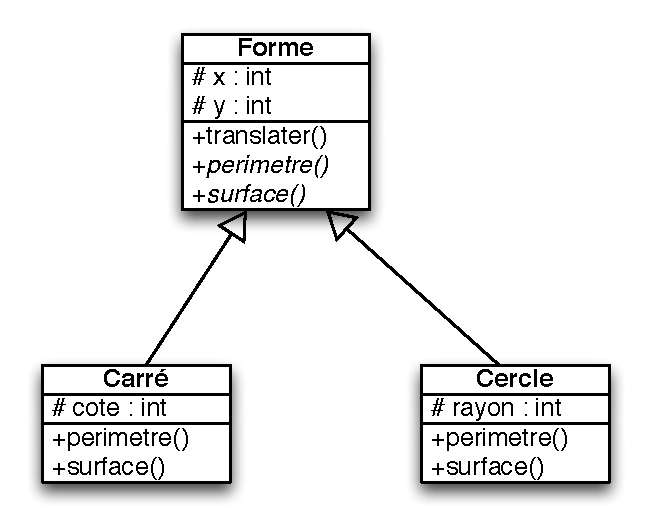
\includegraphics[height=5cm]{fig/forme1.pdf}
\end{center}
\end{frame}
